% !TEX program = xelatex
\documentclass[11pt]{article}
\usepackage{amsmath,amssymb}
\usepackage{mathptmx}
\usepackage[no-math]{fontspec}
\setmainfont{TeX Gyre Termes}
\usepackage{polyglossia}
\setdefaultlanguage{english}
\setotherlanguage{russian}
\newfontfamily\cyrillicfont{FreeSerif}[Ligatures=TeX]
\usepackage[a4paper,margin=2.5cm]{geometry}
\usepackage{setspace}
\setstretch{1.25}
\usepackage{booktabs,array,multirow,tabularx}
\usepackage{graphicx}
\usepackage[font=small,labelfont=bf,skip=4pt]{caption}
\usepackage{pdflscape}
\usepackage[authoryear,round]{natbib}
\usepackage{xcolor}
\definecolor{linkblue}{HTML}{1F4E79}
\usepackage[colorlinks=true,linkcolor=linkblue,citecolor=linkblue,urlcolor=linkblue]{hyperref}
\usepackage{microtype}
\usepackage{enumitem}
\setlist{nosep,leftmargin=*}
\emergencystretch=2.5em
\usepackage[bottom]{footmisc}
\usepackage{float}
\usepackage[section]{placeins}

% Auto-generated by scripts/06_tables_figures.py -- do not edit by hand.
\makeatletter
\newcommand{\val}[1]{\@ifundefined{val@#1}{\textbf{??#1??}}{\csname val@#1\endcsname}}
\makeatother
\expandafter\def\csname val@ADVearlyMax\endcsname{10}
\expandafter\def\csname val@ADVearlyMin\endcsname{7}
\expandafter\def\csname val@ADVlateMax\endcsname{294}
\expandafter\def\csname val@ADVlateMin\endcsname{246}
\expandafter\def\csname val@AdvCrit\endcsname{3.39}
\expandafter\def\csname val@AdvTABVOL\endcsname{2.95}
\expandafter\def\csname val@AdvTRESMOM\endcsname{3.71}
\expandafter\def\csname val@AdvTwoCount\endcsname{4}
\expandafter\def\csname val@AdvTwoCrit\endcsname{3.40}
\expandafter\def\csname val@AdvTwoTABVOL\endcsname{2.34}
\expandafter\def\csname val@AdvTwoTRESMOM\endcsname{3.43}
\expandafter\def\csname val@AlphaABVOL\endcsname{1.38}
\expandafter\def\csname val@AlphaAMIHUD\endcsname{-0.14}
\expandafter\def\csname val@AlphaBETA\endcsname{0.75}
\expandafter\def\csname val@AlphaCOSKEW\endcsname{0.05}
\expandafter\def\csname val@AlphaCVVAL\endcsname{0.97}
\expandafter\def\csname val@AlphaDBETA\endcsname{-0.40}
\expandafter\def\csname val@AlphaDVOL\endcsname{0.26}
\expandafter\def\csname val@AlphaDY\endcsname{0.17}
\expandafter\def\csname val@AlphaHIGH52\endcsname{3.13}
\expandafter\def\csname val@AlphaISKEW\endcsname{0.24}
\expandafter\def\csname val@AlphaIVOL\endcsname{0.91}
\expandafter\def\csname val@AlphaLTR\endcsname{0.07}
\expandafter\def\csname val@AlphaMAX\endcsname{0.12}
\expandafter\def\csname val@AlphaMOM121\endcsname{2.31}
\expandafter\def\csname val@AlphaMOM127\endcsname{1.57}
\expandafter\def\csname val@AlphaMOM61\endcsname{2.22}
\expandafter\def\csname val@AlphaRESMOM\endcsname{1.66}
\expandafter\def\csname val@AlphaSEAS\endcsname{-0.11}
\expandafter\def\csname val@AlphaSIZE\endcsname{0.18}
\expandafter\def\csname val@AlphaSKEW\endcsname{0.56}
\expandafter\def\csname val@AlphaSPREAD\endcsname{-0.90}
\expandafter\def\csname val@AlphaSTR\endcsname{-1.98}
\expandafter\def\csname val@AlphaTURN\endcsname{0.66}
\expandafter\def\csname val@AlphaTVOL\endcsname{0.80}
\expandafter\def\csname val@AlphaZERO\endcsname{-0.30}
\expandafter\def\csname val@BEABVOL\endcsname{67}
\expandafter\def\csname val@BEHIGH52\endcsname{252}
\expandafter\def\csname val@BEMOM121\endcsname{231}
\expandafter\def\csname val@BEMOM127\endcsname{114}
\expandafter\def\csname val@BEMOM61\endcsname{150}
\expandafter\def\csname val@BERESMOM\endcsname{148}
\expandafter\def\csname val@BEfeeABVOL\endcsname{7}
\expandafter\def\csname val@BEfeeHIGH52\endcsname{32}
\expandafter\def\csname val@BEfeeMOM121\endcsname{23}
\expandafter\def\csname val@BEfeeMOM61\endcsname{20}
\expandafter\def\csname val@BEfeeMax\endcsname{32}
\expandafter\def\csname val@BEfeeMin\endcsname{15}
\expandafter\def\csname val@BEfeeRESMOM\endcsname{15}
\expandafter\def\csname val@BEfeeSTR\endcsname{10}
\expandafter\def\csname val@BanTABVOL\endcsname{1.56}
\expandafter\def\csname val@BanTHIGH52\endcsname{4.90}
\expandafter\def\csname val@BanTMOM121\endcsname{3.86}
\expandafter\def\csname val@BanTMOM61\endcsname{3.78}
\expandafter\def\csname val@BanTRESMOM\endcsname{3.64}
\expandafter\def\csname val@BanTSTR\endcsname{2.00}
\expandafter\def\csname val@BanTmax\endcsname{4.90}
\expandafter\def\csname val@BanTmin\endcsname{3.64}
\expandafter\def\csname val@BoardCountsSame\endcsname{unchanged}
\expandafter\def\csname val@BoardCtlHi\endcsname{89}
\expandafter\def\csname val@BoardCtlLo\endcsname{77}
\expandafter\def\csname val@BoardMaxDt\endcsname{0.45}
\expandafter\def\csname val@BoardN\endcsname{23}
\expandafter\def\csname val@BoardPrwABVOL\endcsname{0.047}
\expandafter\def\csname val@BoardSame\endcsname{the same}
\expandafter\def\csname val@BoardStockMonths\endcsname{384}
\expandafter\def\csname val@BoardTABVOL\endcsname{3.38}
\expandafter\def\csname val@BoardValHi\endcsname{18}
\expandafter\def\csname val@BoardValLo\endcsname{5}
\expandafter\def\csname val@BonfCrit\endcsname{3.09}
\expandafter\def\csname val@BootMaxMedian\endcsname{2.12}
\expandafter\def\csname val@CapCovFirst\endcsname{71}
\expandafter\def\csname val@CapFullMax\endcsname{167}
\expandafter\def\csname val@CapFullMin\endcsname{41}
\expandafter\def\csname val@CapHalfMax\endcsname{667}
\expandafter\def\csname val@CapHalfMin\endcsname{165}
\expandafter\def\csname val@CapPostHalfMax\endcsname{6.3}
\expandafter\def\csname val@CapPostHalfMin\endcsname{404}
\expandafter\def\csname val@CapPostMax\endcsname{1.6}
\expandafter\def\csname val@CapPostMin\endcsname{101}
\expandafter\def\csname val@CashNamesMax\endcsname{11}
\expandafter\def\csname val@CompMean\endcsname{2.30}
\expandafter\def\csname val@CompSR\endcsname{1.53}
\expandafter\def\csname val@CompT\endcsname{6.10}
\expandafter\def\csname val@CorrIvolTvol\endcsname{0.95}
\expandafter\def\csname val@CorrMomMom\endcsname{0.87}
\expandafter\def\csname val@CountR1\endcsname{7}
\expandafter\def\csname val@CountR2\endcsname{6}
\expandafter\def\csname val@CountR3\endcsname{6}
\expandafter\def\csname val@CountR4\endcsname{7}
\expandafter\def\csname val@CountR5\endcsname{6}
\expandafter\def\csname val@CountR6\endcsname{5}
\expandafter\def\csname val@CountR7\endcsname{0}
\expandafter\def\csname val@DRmax\endcsname{6}
\expandafter\def\csname val@DRmaxWord\endcsname{six}
\expandafter\def\csname val@DRstockMonths\endcsname{295}
\expandafter\def\csname val@DSRbootPass\endcsname{5}
\expandafter\def\csname val@DataCountsSame\endcsname{unchanged}
\expandafter\def\csname val@DecompData\endcsname{0.20}
\expandafter\def\csname val@DecompDep\endcsname{0.09}
\expandafter\def\csname val@DecompNoise\endcsname{0.19}
\expandafter\def\csname val@DedupChanged\endcsname{44}
\expandafter\def\csname val@DedupDropped\endcsname{50}
\expandafter\def\csname val@DedupDroppedU\endcsname{40}
\expandafter\def\csname val@DedupMaxDt\endcsname{0.06}
\expandafter\def\csname val@DedupOnlyChanged\endcsname{33}
\expandafter\def\csname val@DedupOnlyMaxDt\endcsname{0.04}
\expandafter\def\csname val@DedupSame\endcsname{the same}
\expandafter\def\csname val@DivGroupsAll\endcsname{46}
\expandafter\def\csname val@DivGroupsPairsAll\endcsname{42}
\expandafter\def\csname val@DivGroupsTriples\endcsname{4}
\expandafter\def\csname val@DivPairs\endcsname{40}
\expandafter\def\csname val@DivYahooShare\endcsname{25}
\expandafter\def\csname val@DivYahooShareU\endcsname{15}
\expandafter\def\csname val@DivcalChanged\endcsname{11}
\expandafter\def\csname val@DivcalMaxDt\endcsname{0.03}
\expandafter\def\csname val@DivcalSame\endcsname{the same}
\expandafter\def\csname val@DsrABVOL\endcsname{0.21}
\expandafter\def\csname val@DsrAMIHUD\endcsname{0.00}
\expandafter\def\csname val@DsrBETA\endcsname{0.00}
\expandafter\def\csname val@DsrCOSKEW\endcsname{0.00}
\expandafter\def\csname val@DsrCVVAL\endcsname{0.02}
\expandafter\def\csname val@DsrDBETA\endcsname{0.00}
\expandafter\def\csname val@DsrDVOL\endcsname{0.00}
\expandafter\def\csname val@DsrDY\endcsname{0.00}
\expandafter\def\csname val@DsrHIGH52\endcsname{0.73}
\expandafter\def\csname val@DsrISKEW\endcsname{0.00}
\expandafter\def\csname val@DsrIVOL\endcsname{0.00}
\expandafter\def\csname val@DsrLTR\endcsname{0.00}
\expandafter\def\csname val@DsrMAX\endcsname{0.00}
\expandafter\def\csname val@DsrMOM121\endcsname{0.44}
\expandafter\def\csname val@DsrMOM127\endcsname{0.12}
\expandafter\def\csname val@DsrMOM61\endcsname{0.66}
\expandafter\def\csname val@DsrRESMOM\endcsname{0.57}
\expandafter\def\csname val@DsrSEAS\endcsname{0.00}
\expandafter\def\csname val@DsrSIZE\endcsname{0.00}
\expandafter\def\csname val@DsrSKEW\endcsname{0.00}
\expandafter\def\csname val@DsrSPREAD\endcsname{0.00}
\expandafter\def\csname val@DsrSTR\endcsname{0.00}
\expandafter\def\csname val@DsrTURN\endcsname{0.00}
\expandafter\def\csname val@DsrTVOL\endcsname{0.00}
\expandafter\def\csname val@DsrZERO\endcsname{0.00}
\expandafter\def\csname val@EBmuzero\endcsname{0.20}
\expandafter\def\csname val@EBncPos\endcsname{12}
\expandafter\def\csname val@EBnineNpos\endcsname{13}
\expandafter\def\csname val@EBnineSame\endcsname{the same}
\expandafter\def\csname val@EBnrep\endcsname{13}
\expandafter\def\csname val@EBpostSDmed\endcsname{0.17}
\expandafter\def\csname val@EBrate\endcsname{52}
\expandafter\def\csname val@EBtauc\endcsname{0.35}
\expandafter\def\csname val@EBtauw\endcsname{0.11}
\expandafter\def\csname val@EigOne\endcsname{8.26}
\expandafter\def\csname val@EigShare\endcsname{33}
\expandafter\def\csname val@FMmaxTmulti\endcsname{1.83}
\expandafter\def\csname val@FMtABVOLB\endcsname{1.02}
\expandafter\def\csname val@FMtHIGHB\endcsname{1.76}
\expandafter\def\csname val@FMtHIGHuni\endcsname{6.23}
\expandafter\def\csname val@FMtMOMA\endcsname{5.22}
\expandafter\def\csname val@FMtMOMB\endcsname{2.09}
\expandafter\def\csname val@FMtSTRA\endcsname{-3.46}
\expandafter\def\csname val@FMtSTRB\endcsname{-2.37}
\expandafter\def\csname val@FWERnp\endcsname{6.5}
\expandafter\def\csname val@FWERpar\endcsname{6.2}
\expandafter\def\csname val@FWERreps\endcsname{1000}
\expandafter\def\csname val@FWalphaBoot\endcsname{0.030}
\expandafter\def\csname val@FWalphaPar\endcsname{0.044}
\expandafter\def\csname val@FWalphaStar\endcsname{0.03}
\expandafter\def\csname val@FWcritStar\endcsname{3.60}
\expandafter\def\csname val@FWholmBoot\endcsname{9.8}
\expandafter\def\csname val@FWholmPar\endcsname{8.0}
\expandafter\def\csname val@FWpAbvol\endcsname{0.033}
\expandafter\def\csname val@FWreps\endcsname{4{,}000}
\expandafter\def\csname val@FWrwBoot\endcsname{7.3}
\expandafter\def\csname val@FWrwBootHi\endcsname{8.2}
\expandafter\def\csname val@FWrwBootLo\endcsname{6.6}
\expandafter\def\csname val@FWrwPar\endcsname{5.8}
\expandafter\def\csname val@FWrwParHi\endcsname{6.5}
\expandafter\def\csname val@FWrwParLo\endcsname{5.1}
\expandafter\def\csname val@FWtthreeBoot\endcsname{11.5}
\expandafter\def\csname val@FWtthreePar\endcsname{9.7}
\expandafter\def\csname val@FeeTenTABVOL\endcsname{-0.68}
\expandafter\def\csname val@FeeTenTHIGH52\endcsname{3.52}
\expandafter\def\csname val@FeeTenTMOM121\endcsname{2.23}
\expandafter\def\csname val@FeeTenTMOM61\endcsname{1.96}
\expandafter\def\csname val@FeeTenTRESMOM\endcsname{1.23}
\expandafter\def\csname val@FeeTenTSTR\endcsname{-0.02}
\expandafter\def\csname val@FloorFirst\endcsname{26}
\expandafter\def\csname val@FloorLast\endcsname{508}
\expandafter\def\csname val@GlobalNullP\endcsname{0.0002}
\expandafter\def\csname val@IdxBases\endcsname{60}
\expandafter\def\csname val@IdxFallbackABVOL\endcsname{19}
\expandafter\def\csname val@IdxMissBases\endcsname{52}
\expandafter\def\csname val@IdxMissMax\endcsname{4}
\expandafter\def\csname val@IdxMissMaxWord\endcsname{four}
\expandafter\def\csname val@IdxTABVOL\endcsname{0.14}
\expandafter\def\csname val@IdxTHIGH52\endcsname{4.32}
\expandafter\def\csname val@IdxTMOM121\endcsname{3.67}
\expandafter\def\csname val@IdxTMOM61\endcsname{2.46}
\expandafter\def\csname val@IdxTRESMOM\endcsname{3.21}
\expandafter\def\csname val@IdxTSTR\endcsname{1.09}
\expandafter\def\csname val@IdxTmax\endcsname{4.32}
\expandafter\def\csname val@IdxTmin\endcsname{2.46}
\expandafter\def\csname val@IdxWinTmax\endcsname{5.32}
\expandafter\def\csname val@IdxWinTmin\endcsname{3.72}
\expandafter\def\csname val@ImpLongHIGH\endcsname{1.53}
\expandafter\def\csname val@ImpLongTHIGH\endcsname{6.65}
\expandafter\def\csname val@ImpShareMax\endcsname{52}
\expandafter\def\csname val@ImpShareMin\endcsname{37}
\expandafter\def\csname val@ImpShortHIGH\endcsname{1.55}
\expandafter\def\csname val@ImpShortTHIGH\endcsname{4.67}
\expandafter\def\csname val@ImpactZeroMonths\endcsname{0}
\expandafter\def\csname val@MeanABVOL\endcsname{1.40}
\expandafter\def\csname val@MeanAMIHUD\endcsname{-0.16}
\expandafter\def\csname val@MeanAbsCorr\endcsname{0.29}
\expandafter\def\csname val@MeanAbsSTR\endcsname{1.96}
\expandafter\def\csname val@MeanBETA\endcsname{0.69}
\expandafter\def\csname val@MeanCOSKEW\endcsname{0.06}
\expandafter\def\csname val@MeanCVVAL\endcsname{0.98}
\expandafter\def\csname val@MeanDBETA\endcsname{-0.35}
\expandafter\def\csname val@MeanDVOL\endcsname{0.24}
\expandafter\def\csname val@MeanDY\endcsname{0.16}
\expandafter\def\csname val@MeanHIGH52\endcsname{3.08}
\expandafter\def\csname val@MeanISKEW\endcsname{0.24}
\expandafter\def\csname val@MeanIVOL\endcsname{0.85}
\expandafter\def\csname val@MeanLTR\endcsname{0.08}
\expandafter\def\csname val@MeanMAX\endcsname{0.06}
\expandafter\def\csname val@MeanMOM121\endcsname{2.28}
\expandafter\def\csname val@MeanMOM127\endcsname{1.54}
\expandafter\def\csname val@MeanMOM61\endcsname{2.19}
\expandafter\def\csname val@MeanRESMOM\endcsname{1.64}
\expandafter\def\csname val@MeanSEAS\endcsname{-0.12}
\expandafter\def\csname val@MeanSIZE\endcsname{0.18}
\expandafter\def\csname val@MeanSKEW\endcsname{0.56}
\expandafter\def\csname val@MeanSPREAD\endcsname{-0.83}
\expandafter\def\csname val@MeanSTR\endcsname{-1.96}
\expandafter\def\csname val@MeanTURN\endcsname{0.62}
\expandafter\def\csname val@MeanTVOL\endcsname{0.72}
\expandafter\def\csname val@MeanZERO\endcsname{-0.32}
\expandafter\def\csname val@MechCritLeight\endcsname{3.50}
\expandafter\def\csname val@MechCritLtwelve\endcsname{3.67}
\expandafter\def\csname val@MechIidCrit\endcsname{3.28}
\expandafter\def\csname val@MechIidPthree\endcsname{0.0036}
\expandafter\def\csname val@MechIidSD\endcsname{1.034}
\expandafter\def\csname val@MechKurtMed\endcsname{3.19}
\expandafter\def\csname val@MechNormalScores\endcsname{3.47}
\expandafter\def\csname val@MechPosAC\endcsname{72}
\expandafter\def\csname val@MechRescaled\endcsname{3.11}
\expandafter\def\csname val@MechRetKurtMed\endcsname{6.5}
\expandafter\def\csname val@MechSDmax\endcsname{1.25}
\expandafter\def\csname val@MechSDmed\endcsname{1.07}
\expandafter\def\csname val@MechSDmin\endcsname{0.95}
\expandafter\def\csname val@MechSidakNeff\endcsname{2.93}
\expandafter\def\csname val@MechTratioLtwelve\endcsname{4}
\expandafter\def\csname val@MktExcess\endcsname{0.10}
\expandafter\def\csname val@NallMean\endcsname{232}
\expandafter\def\csname val@NeffLiJi\endcsname{15}
\expandafter\def\csname val@NeffNyholt\endcsname{22.0}
\expandafter\def\csname val@NetMeanABVOL\endcsname{0.56}
\expandafter\def\csname val@NetMeanHIGH52\endcsname{2.63}
\expandafter\def\csname val@NetMeanMOM121\endcsname{1.90}
\expandafter\def\csname val@NetMeanMOM127\endcsname{1.02}
\expandafter\def\csname val@NetMeanMOM61\endcsname{1.63}
\expandafter\def\csname val@NetMeanRESMOM\endcsname{1.24}
\expandafter\def\csname val@NetRWcount\endcsname{4}
\expandafter\def\csname val@NetTABVOL\endcsname{1.40}
\expandafter\def\csname val@NetTHIGH52\endcsname{5.15}
\expandafter\def\csname val@NetTMOM121\endcsname{3.97}
\expandafter\def\csname val@NetTMOM127\endcsname{2.15}
\expandafter\def\csname val@NetTMOM61\endcsname{4.00}
\expandafter\def\csname val@NetTRESMOM\endcsname{3.75}
\expandafter\def\csname val@NetTwoABVOL\endcsname{-0.66}
\expandafter\def\csname val@NetTwoHIGH52\endcsname{4.22}
\expandafter\def\csname val@NetTwoMOM121\endcsname{3.20}
\expandafter\def\csname val@NetTwoMOM127\endcsname{1.07}
\expandafter\def\csname val@NetTwoMOM61\endcsname{2.64}
\expandafter\def\csname val@NetTwoRESMOM\endcsname{2.56}
\expandafter\def\csname val@NormMaxCrit\endcsname{3.08}
\expandafter\def\csname val@NsplitEvents\endcsname{14}
\expandafter\def\csname val@NsplitPit\endcsname{6}
\expandafter\def\csname val@OLSseMed\endcsname{0.41}
\expandafter\def\csname val@PBO\endcsname{0.032}
\expandafter\def\csname val@PBOT\endcsname{175}
\expandafter\def\csname val@PBOabvol\endcsname{14}
\expandafter\def\csname val@PBOhigh\endcsname{47}
\expandafter\def\csname val@PBOmom\endcsname{84}
\expandafter\def\csname val@PBOrankMed\endcsname{22}
\expandafter\def\csname val@PBOrankWord\endcsname{fourth}
\expandafter\def\csname val@PBOsplits\endcsname{12870}
\expandafter\def\csname val@PBOtopfive\endcsname{78}
\expandafter\def\csname val@PayersMean\endcsname{60}
\expandafter\def\csname val@PowRWsr0p5\endcsname{0.13}
\expandafter\def\csname val@PowRWsr0p75\endcsname{0.39}
\expandafter\def\csname val@PowRWsr1p0\endcsname{0.72}
\expandafter\def\csname val@PowRWsr1p25\endcsname{0.91}
\expandafter\def\csname val@PowTsr0p5\endcsname{0.50}
\expandafter\def\csname val@PowTsr0p75\endcsname{0.81}
\expandafter\def\csname val@PowTsr1p0\endcsname{0.96}
\expandafter\def\csname val@PowTsr1p25\endcsname{0.99}
\expandafter\def\csname val@PrwABVOL\endcsname{0.033}
\expandafter\def\csname val@PrwAMIHUD\endcsname{0.999}
\expandafter\def\csname val@PrwBETA\endcsname{0.773}
\expandafter\def\csname val@PrwCOSKEW\endcsname{0.999}
\expandafter\def\csname val@PrwCVVAL\endcsname{0.137}
\expandafter\def\csname val@PrwDBETA\endcsname{0.984}
\expandafter\def\csname val@PrwDVOL\endcsname{0.995}
\expandafter\def\csname val@PrwDY\endcsname{0.999}
\expandafter\def\csname val@PrwHIGH52\endcsname{0.000}
\expandafter\def\csname val@PrwISKEW\endcsname{0.996}
\expandafter\def\csname val@PrwIVOL\endcsname{0.575}
\expandafter\def\csname val@PrwLTR\endcsname{0.999}
\expandafter\def\csname val@PrwMAX\endcsname{0.999}
\expandafter\def\csname val@PrwMOM121\endcsname{0.002}
\expandafter\def\csname val@PrwMOM127\endcsname{0.058}
\expandafter\def\csname val@PrwMOM61\endcsname{0.001}
\expandafter\def\csname val@PrwRESMOM\endcsname{0.001}
\expandafter\def\csname val@PrwSEAS\endcsname{0.999}
\expandafter\def\csname val@PrwSIZE\endcsname{0.999}
\expandafter\def\csname val@PrwSKEW\endcsname{0.787}
\expandafter\def\csname val@PrwSPREAD\endcsname{0.644}
\expandafter\def\csname val@PrwSTR\endcsname{0.001}
\expandafter\def\csname val@PrwTURN\endcsname{0.773}
\expandafter\def\csname val@PrwTVOL\endcsname{0.787}
\expandafter\def\csname val@PrwZERO\endcsname{0.995}
\expandafter\def\csname val@QiidCorrL12\endcsname{3.52}
\expandafter\def\csname val@QiidCorrL4\endcsname{3.19}
\expandafter\def\csname val@QiidCorrL8\endcsname{3.35}
\expandafter\def\csname val@QiidIndepL4\endcsname{3.28}
\expandafter\def\csname val@QnormCorr\endcsname{2.99}
\expandafter\def\csname val@QnormIndep\endcsname{3.08}
\expandafter\def\csname val@RWcapm\endcsname{6}
\expandafter\def\csname val@RWcosts\endcsname{4}
\expandafter\def\csname val@RWcrit\endcsname{3.39}
\expandafter\def\csname val@RWcritB12\endcsname{3.55}
\expandafter\def\csname val@RWcritB3\endcsname{3.31}
\expandafter\def\csname val@RWcritPost\endcsname{3.93}
\expandafter\def\csname val@RWcritPre\endcsname{3.47}
\expandafter\def\csname val@RWextrans\endcsname{6}
\expandafter\def\csname val@RWlag1\endcsname{4}
\expandafter\def\csname val@RWpit\endcsname{5}
\expandafter\def\csname val@RWpriceonly\endcsname{4}
\expandafter\def\csname val@RWregpost\endcsname{0}
\expandafter\def\csname val@RWregpre\endcsname{4}
\expandafter\def\csname val@RWterciles\endcsname{6}
\expandafter\def\csname val@RWu100ord\endcsname{6}
\expandafter\def\csname val@RWu50\endcsname{3}
\expandafter\def\csname val@RWuall\endcsname{1}
\expandafter\def\csname val@RWvw\endcsname{4}
\expandafter\def\csname val@RegBHsig\endcsname{0}
\expandafter\def\csname val@RegMinPdvol\endcsname{0.16}
\expandafter\def\csname val@RegMomHi\endcsname{0.74}
\expandafter\def\csname val@RegMomLo\endcsname{-1.97}
\expandafter\def\csname val@RegMomPost\endcsname{1.87}
\expandafter\def\csname val@RegMomPre\endcsname{2.49}
\expandafter\def\csname val@RegMomT\endcsname{-0.88}
\expandafter\def\csname val@RegPostAMIHUD\endcsname{0.84}
\expandafter\def\csname val@RegPostBETA\endcsname{1.23}
\expandafter\def\csname val@RegPostDVOL\endcsname{1.37}
\expandafter\def\csname val@RegPostHIGH52\endcsname{2.92}
\expandafter\def\csname val@RegPostMOM61\endcsname{1.39}
\expandafter\def\csname val@RegPostSEAS\endcsname{0.51}
\expandafter\def\csname val@RegPostSTR\endcsname{-1.61}
\expandafter\def\csname val@RegPostZERO\endcsname{1.07}
\expandafter\def\csname val@RegPreAMIHUD\endcsname{-0.60}
\expandafter\def\csname val@RegPreBETA\endcsname{0.44}
\expandafter\def\csname val@RegPreDVOL\endcsname{-0.27}
\expandafter\def\csname val@RegPreHIGH52\endcsname{3.15}
\expandafter\def\csname val@RegPreMOM61\endcsname{2.55}
\expandafter\def\csname val@RegPreSEAS\endcsname{-0.40}
\expandafter\def\csname val@RegPreSTR\endcsname{-2.12}
\expandafter\def\csname val@RegPreZERO\endcsname{-0.94}
\expandafter\def\csname val@RegRawPdvol\endcsname{0.013}
\expandafter\def\csname val@RegTdAMIHUD\endcsname{1.75}
\expandafter\def\csname val@RegTdBETA\endcsname{0.97}
\expandafter\def\csname val@RegTdDVOL\endcsname{2.49}
\expandafter\def\csname val@RegTdHIGH52\endcsname{-0.23}
\expandafter\def\csname val@RegTdMOM61\endcsname{-1.61}
\expandafter\def\csname val@RegTdSEAS\endcsname{1.67}
\expandafter\def\csname val@RegTdSTR\endcsname{0.55}
\expandafter\def\csname val@RegTdZERO\endcsname{2.49}
\expandafter\def\csname val@RegTpostAMIHUD\endcsname{1.07}
\expandafter\def\csname val@RegTpostBETA\endcsname{2.06}
\expandafter\def\csname val@RegTpostDVOL\endcsname{2.16}
\expandafter\def\csname val@RegTpostHIGH52\endcsname{3.70}
\expandafter\def\csname val@RegTpostMOM61\endcsname{2.37}
\expandafter\def\csname val@RegTpostSEAS\endcsname{1.22}
\expandafter\def\csname val@RegTpostSTR\endcsname{-2.04}
\expandafter\def\csname val@RegTpostZERO\endcsname{1.71}
\expandafter\def\csname val@RegTpreAMIHUD\endcsname{-1.36}
\expandafter\def\csname val@RegTpreBETA\endcsname{0.73}
\expandafter\def\csname val@RegTpreDVOL\endcsname{-0.78}
\expandafter\def\csname val@RegTpreHIGH52\endcsname{4.80}
\expandafter\def\csname val@RegTpreMOM61\endcsname{4.92}
\expandafter\def\csname val@RegTpreSEAS\endcsname{-1.12}
\expandafter\def\csname val@RegTpreSTR\endcsname{-4.45}
\expandafter\def\csname val@RegTpreZERO\endcsname{-1.70}
\expandafter\def\csname val@RegZooDelta\endcsname{0.20}
\expandafter\def\csname val@RegZooHi\endcsname{0.64}
\expandafter\def\csname val@RegZooLo\endcsname{-0.23}
\expandafter\def\csname val@RegZooMDE\endcsname{0.62}
\expandafter\def\csname val@RegZooPost\endcsname{0.70}
\expandafter\def\csname val@RegZooPre\endcsname{0.49}
\expandafter\def\csname val@RegZooT\endcsname{0.92}
\expandafter\def\csname val@RegZooTpost\endcsname{4.24}
\expandafter\def\csname val@RegZooTpre\endcsname{3.17}
\expandafter\def\csname val@SMBmean\endcsname{0.76}
\expandafter\def\csname val@SMBt\endcsname{1.69}
\expandafter\def\csname val@SRABVOL\endcsname{1.02}
\expandafter\def\csname val@SRAMIHUD\endcsname{-0.09}
\expandafter\def\csname val@SRBETA\endcsname{0.37}
\expandafter\def\csname val@SRCOSKEW\endcsname{0.06}
\expandafter\def\csname val@SRCVVAL\endcsname{0.63}
\expandafter\def\csname val@SRDBETA\endcsname{-0.22}
\expandafter\def\csname val@SRDVOL\endcsname{0.16}
\expandafter\def\csname val@SRDY\endcsname{0.12}
\expandafter\def\csname val@SRHIGH52\endcsname{1.44}
\expandafter\def\csname val@SRISKEW\endcsname{0.16}
\expandafter\def\csname val@SRIVOL\endcsname{0.48}
\expandafter\def\csname val@SRLTR\endcsname{0.05}
\expandafter\def\csname val@SRMAX\endcsname{0.04}
\expandafter\def\csname val@SRMOM121\endcsname{1.17}
\expandafter\def\csname val@SRMOM127\endcsname{0.84}
\expandafter\def\csname val@SRMOM61\endcsname{1.34}
\expandafter\def\csname val@SRRESMOM\endcsname{1.28}
\expandafter\def\csname val@SRSEAS\endcsname{-0.10}
\expandafter\def\csname val@SRSIZE\endcsname{0.13}
\expandafter\def\csname val@SRSKEW\endcsname{0.38}
\expandafter\def\csname val@SRSPREAD\endcsname{-0.42}
\expandafter\def\csname val@SRSTR\endcsname{-1.23}
\expandafter\def\csname val@SRTURN\endcsname{0.46}
\expandafter\def\csname val@SRTVOL\endcsname{0.39}
\expandafter\def\csname val@SRZERO\endcsname{-0.20}
\expandafter\def\csname val@SRsurvMax\endcsname{1.44}
\expandafter\def\csname val@SRsurvMin\endcsname{1.02}
\expandafter\def\csname val@SRzeroAll\endcsname{1.74}
\expandafter\def\csname val@SRzeroBoot\endcsname{0.50}
\expandafter\def\csname val@SRzeroN\endcsname{1.23}
\expandafter\def\csname val@SRzeroNeff\endcsname{1.09}
\expandafter\def\csname val@STRdiffM\endcsname{2.28}
\expandafter\def\csname val@STRdiffT\endcsname{2.84}
\expandafter\def\csname val@STRhighM\endcsname{1.04}
\expandafter\def\csname val@STRhighT\endcsname{1.58}
\expandafter\def\csname val@STRlowM\endcsname{-1.23}
\expandafter\def\csname val@STRlowT\endcsname{-1.90}
\expandafter\def\csname val@SeedCritMax\endcsname{3.45}
\expandafter\def\csname val@SeedCritMin\endcsname{3.39}
\expandafter\def\csname val@SeedPabvolMax\endcsname{0.039}
\expandafter\def\csname val@SeedPabvolMin\endcsname{0.033}
\expandafter\def\csname val@SeedSame\endcsname{the same}
\expandafter\def\csname val@SpanTABVOL\endcsname{1.93}
\expandafter\def\csname val@SpanTHIGH52\endcsname{2.33}
\expandafter\def\csname val@SpanTMOM121\endcsname{-0.92}
\expandafter\def\csname val@SpanTMOM61\endcsname{0.80}
\expandafter\def\csname val@SpanTRESMOM\endcsname{2.27}
\expandafter\def\csname val@SpanTwoTMOM121\endcsname{-0.81}
\expandafter\def\csname val@SpanTwoTMOM61\endcsname{0.47}
\expandafter\def\csname val@SurvCorrAbvolMax\endcsname{0.19}
\expandafter\def\csname val@SurvCorrMax\endcsname{0.78}
\expandafter\def\csname val@SurvCorrMin\endcsname{0.40}
\expandafter\def\csname val@SurvEigShare\endcsname{73}
\expandafter\def\csname val@TABVOL\endcsname{3.52}
\expandafter\def\csname val@TAMIHUD\endcsname{-0.39}
\expandafter\def\csname val@TBETA\endcsname{1.52}
\expandafter\def\csname val@TCOSKEW\endcsname{0.21}
\expandafter\def\csname val@TCVVAL\endcsname{2.79}
\expandafter\def\csname val@TDBETA\endcsname{-0.89}
\expandafter\def\csname val@TDVOL\endcsname{0.70}
\expandafter\def\csname val@TDY\endcsname{0.37}
\expandafter\def\csname val@THIGH52\endcsname{6.07}
\expandafter\def\csname val@TISKEW\endcsname{0.59}
\expandafter\def\csname val@TIVOL\endcsname{1.85}
\expandafter\def\csname val@TLTR\endcsname{0.19}
\expandafter\def\csname val@TMAX\endcsname{0.13}
\expandafter\def\csname val@TMOM121\endcsname{4.72}
\expandafter\def\csname val@TMOM127\endcsname{3.24}
\expandafter\def\csname val@TMOM61\endcsname{5.33}
\expandafter\def\csname val@TOABVOL\endcsname{2.08}
\expandafter\def\csname val@TOHIGH52\endcsname{1.23}
\expandafter\def\csname val@TOMOM121\endcsname{0.99}
\expandafter\def\csname val@TOMOM127\endcsname{1.35}
\expandafter\def\csname val@TOMOM61\endcsname{1.46}
\expandafter\def\csname val@TORESMOM\endcsname{1.11}
\expandafter\def\csname val@TRESMOM\endcsname{4.90}
\expandafter\def\csname val@TSEAS\endcsname{-0.41}
\expandafter\def\csname val@TSIZE\endcsname{0.41}
\expandafter\def\csname val@TSKEW\endcsname{1.46}
\expandafter\def\csname val@TSPREAD\endcsname{-1.74}
\expandafter\def\csname val@TSTR\endcsname{-4.96}
\expandafter\def\csname val@TTURN\endcsname{1.52}
\expandafter\def\csname val@TTVOL\endcsname{1.46}
\expandafter\def\csname val@TZERO\endcsname{-0.70}
\expandafter\def\csname val@TabsSTR\endcsname{4.96}
\expandafter\def\csname val@TalphaABVOL\endcsname{3.75}
\expandafter\def\csname val@TalphaAMIHUD\endcsname{-0.37}
\expandafter\def\csname val@TalphaBETA\endcsname{1.74}
\expandafter\def\csname val@TalphaCOSKEW\endcsname{0.18}
\expandafter\def\csname val@TalphaCVVAL\endcsname{2.81}
\expandafter\def\csname val@TalphaDBETA\endcsname{-1.04}
\expandafter\def\csname val@TalphaDVOL\endcsname{0.81}
\expandafter\def\csname val@TalphaDY\endcsname{0.44}
\expandafter\def\csname val@TalphaHIGH52\endcsname{5.95}
\expandafter\def\csname val@TalphaISKEW\endcsname{0.62}
\expandafter\def\csname val@TalphaIVOL\endcsname{2.18}
\expandafter\def\csname val@TalphaLTR\endcsname{0.16}
\expandafter\def\csname val@TalphaMAX\endcsname{0.27}
\expandafter\def\csname val@TalphaMOM121\endcsname{4.98}
\expandafter\def\csname val@TalphaMOM127\endcsname{3.46}
\expandafter\def\csname val@TalphaMOM61\endcsname{5.62}
\expandafter\def\csname val@TalphaRESMOM\endcsname{5.01}
\expandafter\def\csname val@TalphaSEAS\endcsname{-0.40}
\expandafter\def\csname val@TalphaSIZE\endcsname{0.40}
\expandafter\def\csname val@TalphaSKEW\endcsname{1.47}
\expandafter\def\csname val@TalphaSPREAD\endcsname{-2.01}
\expandafter\def\csname val@TalphaSTR\endcsname{-4.76}
\expandafter\def\csname val@TalphaTURN\endcsname{1.93}
\expandafter\def\csname val@TalphaTVOL\endcsname{1.87}
\expandafter\def\csname val@TalphaZERO\endcsname{-0.68}
\expandafter\def\csname val@TermCVVALshort\endcsname{18}
\expandafter\def\csname val@TermCVVALtot\endcsname{21}
\expandafter\def\csname val@TermCharged\endcsname{45}
\expandafter\def\csname val@TermChargedNone\endcsname{2}
\expandafter\def\csname val@TermChargedNoneWord\endcsname{two}
\expandafter\def\csname val@TermChargedPartial\endcsname{43}
\expandafter\def\csname val@TermHIGHlong\endcsname{12}
\expandafter\def\csname val@TermHIGHshort\endcsname{20}
\expandafter\def\csname val@TermNone\endcsname{12}
\expandafter\def\csname val@TermNoneAfter\endcsname{10}
\expandafter\def\csname val@TermPartial\endcsname{43}
\expandafter\def\csname val@TermPartialBelow\endcsname{11}
\expandafter\def\csname val@TermPartialMean\endcsname{-13}
\expandafter\def\csname val@TermRESMOMlong\endcsname{9}
\expandafter\def\csname val@TermRESMOMshort\endcsname{8}
\expandafter\def\csname val@TermSecids\endcsname{45}
\expandafter\def\csname val@TermShortMoreWord\endcsname{three}
\expandafter\def\csname val@TermSusp\endcsname{3}
\expandafter\def\csname val@TermSuspWord\endcsname{three}
\expandafter\def\csname val@TermTotal\endcsname{55}
\expandafter\def\csname val@TwoFrankIVOL\endcsname{0.98}
\expandafter\def\csname val@TwoFrankRESMOM\endcsname{0.93}
\expandafter\def\csname val@TwoFtIVOL\endcsname{1.74}
\expandafter\def\csname val@TwoFtRESMOM\endcsname{4.09}
\expandafter\def\csname val@UfiftyTABVOL\endcsname{2.09}
\expandafter\def\csname val@UfiftyTHIGH52\endcsname{3.87}
\expandafter\def\csname val@UfiftyTMOM121\endcsname{3.38}
\expandafter\def\csname val@UfiftyTMOM61\endcsname{2.81}
\expandafter\def\csname val@UfiftyTRESMOM\endcsname{3.13}
\expandafter\def\csname val@UfiftyTSTR\endcsname{1.19}
\expandafter\def\csname val@UfiftyTmax\endcsname{3.87}
\expandafter\def\csname val@UfiftyTmin\endcsname{2.81}
\expandafter\def\csname val@UhundDiffM\endcsname{0.58}
\expandafter\def\csname val@UhundDiffT\endcsname{1.15}
\expandafter\def\csname val@UhundHighTurnM\endcsname{1.96}
\expandafter\def\csname val@UhundHighTurnT\endcsname{3.54}
\expandafter\def\csname val@UhundLowTurnM\endcsname{1.38}
\expandafter\def\csname val@UhundLowTurnT\endcsname{3.16}
\expandafter\def\csname val@UhundTopTurn\endcsname{49}
\expandafter\def\csname val@YahooEarlyChanged\endcsname{199}
\expandafter\def\csname val@YahooEarlyMaxDt\endcsname{0.23}
\expandafter\def\csname val@YahooEarlySame\endcsname{the same}
\expandafter\def\csname val@YahooLateChanged\endcsname{197}
\expandafter\def\csname val@YahooLateMaxDt\endcsname{0.38}
\expandafter\def\csname val@YahooLateSame\endcsname{the same}
\expandafter\def\csname val@YahooMaxDt\endcsname{0.37}
\expandafter\def\csname val@YahooMaxDtBaseT\endcsname{-0.41}
\expandafter\def\csname val@YahooMaxDtId\endcsname{SEAS}
\expandafter\def\csname val@YahooMaxDtSurv\endcsname{0.07}

% Appended by scripts/07_validation_stats.py
\expandafter\def\csname val@ContNetMean\endcsname{0.82}
\expandafter\def\csname val@ContNetT\endcsname{2.00}
\expandafter\def\csname val@ContTurnover\endcsname{3.10}
\expandafter\def\csname val@NbadPrints\endcsname{18}
\expandafter\def\csname val@NdeadAll\endcsname{164}
\expandafter\def\csname val@NdeadHundred\endcsname{90}
\expandafter\def\csname val@NdeadHundredPct\endcsname{34}
\expandafter\def\csname val@NdictDelisted\endcsname{758}
\expandafter\def\csname val@NdictSecids\endcsname{1034}
\expandafter\def\csname val@NdivSkipAfterlast\endcsname{1}
\expandafter\def\csname val@NdivSkipBeforefirst\endcsname{121}
\expandafter\def\csname val@NdivSkipGap\endcsname{262}
\expandafter\def\csname val@NdivSkipNonrub\endcsname{30}
\expandafter\def\csname val@NdivUsed\endcsname{2624}
\expandafter\def\csname val@NeverAll\endcsname{423}
\expandafter\def\csname val@NeverHundred\endcsname{261}
\expandafter\def\csname val@NformMonths\endcsname{177}
\expandafter\def\csname val@NpriceSecids\endcsname{1012}
\expandafter\def\csname val@NrenamedHundred\endcsname{10}
\expandafter\def\csname val@NsplitSecids\endcsname{14}
\expandafter\def\csname val@PanelRowsAll\endcsname{40941}
\expandafter\def\csname val@PanelRowsHundred\endcsname{17700}
\expandafter\def\csname val@ValCorr\endcsname{0.988}
\expandafter\def\csname val@ValDiffAnn\endcsname{0.37}
\expandafter\def\csname val@ValT\endcsname{165}
\expandafter\def\csname val@WorstAbsHIGH52\endcsname{33.3}
\expandafter\def\csname val@WorstAbsMOM121\endcsname{44.9}
\expandafter\def\csname val@WorstAbsMOM61\endcsname{16.6}
\expandafter\def\csname val@WorstHIGH52\endcsname{-33.3}
\expandafter\def\csname val@WorstMOM121\endcsname{-44.9}
\expandafter\def\csname val@WorstMOM61\endcsname{-16.6}
\expandafter\def\csname val@WorstMonthHIGH52\endcsname{2015-02}
\expandafter\def\csname val@WorstMonthMOM121\endcsname{2015-02}
\expandafter\def\csname val@WorstMonthMOM61\endcsname{2015-02}


\newcommand{\tabnote}[1]{\par\vspace{3pt}\begin{minipage}{\linewidth}\footnotesize\setstretch{1.0}#1\end{minipage}}
\newcommand{\RW}{Romano--Wolf}
\newcommand{\cmark}{\checkmark}

\title{How Many Factors Are Real on the Moscow Exchange?\\[4pt]
\large A Pre-Specified Multiple-Testing Study of the Russian Factor Zoo}
\author{Sergey Nefedov\thanks{Lomonosov Moscow State University. ORCID: 0009-0008-8929-4848.
The analysis plan was frozen, hashed and committed to version control before any characteristic was computed
(Section~\ref{sec:design}); code, plan and factor return series: \url{https://github.com/Sergpreneur/moex-factor-zoo}.}}
\date{October 2026}

\begin{document}
\maketitle
\thispagestyle{empty}

\begin{abstract}
\noindent
Do the return anomalies documented in developed markets exist on the Moscow Exchange once the number of tests is
taken into account? I test implementations of 25 price-, trading- and payout-based predictors on MOEX-listed equities (holding
months 2012:01--2026:09), with data free of survivorship bias for shares but covering depositary receipts only in part,
under a protocol fixed before estimation, and evaluate each under
a ladder of seven significance criteria. Seven characteristics clear $|t|>1.96$ in the predicted direction; five
survive the \RW{} stepdown, whose bootstrap critical value (\val{RWcrit}) exceeds both the Harvey--Liu--Zhu hurdle
and the normal-theory Bonferroni bound: with fifteen years of monthly data, autocorrelation-robust $t$-statistics are
more dispersed than the normal distribution that normal-theory corrections assume. Four survivors are closely related
measures of intermediate-horizon momentum---nearness to the 52-week high, six- and twelve-month and residual
momentum---and are largely redundant rather than four independent discoveries; the fifth, a high-volume premium, is
fragile. The implemented
low-risk, liquidity, size, skewness, seasonality and dividend-yield signals do not survive, but premia with annual Sharpe
ratios below about one would often go undetected in a sample of this length. The one-month reversal is reversed: among
liquid shares last month's winners keep winning ($t=\val{TSTR}$ against the reversal hypothesis). Momentum remains
significant net of estimated spread costs, with short legs restricted to index shares and under bounds for unobserved
delisting losses, but its capacity in equal-weighted form is small. After the 2022 exclusion of foreign investors no
premium changes significantly once the 25 differences are corrected for multiplicity, yet the confidence intervals
admit large changes in either direction.

\medskip\noindent
\textbf{JEL:} G12, G14, G15, C12. \quad
\textbf{Keywords:} factor zoo, multiple testing, Romano--Wolf, replication, momentum, Russian stock market, MOEX.
\end{abstract}

\clearpage
\thispagestyle{empty}
\begin{russian}
\begin{abstract}
\sloppy\noindent
Существуют ли на Московской бирже аномалии доходности, найденные на развитых рынках, если учесть число проверяемых
гипотез? В работе проверяются реализации 25 предикторов доходности, основанных на ценах, торговой активности и
дивидендах, на выборке бумаг Мосбиржи (месяцы удержания 2012:01--2026:09), которая свободна от ошибки выжившего в части
акций, но лишь частично охватывает депозитарные расписки, по протоколу,
зафиксированному до оценивания; каждый оценивается по лестнице из семи критериев значимости. Порог $|t|>1{,}96$ в
предсказанном направлении проходят семь характеристик; пошаговую процедуру Романо--Вольфа выдерживают пять, причём её
бутстреп-критическое значение (3,39) выше и порога Харви--Лю--Чжу, и нормального порога Бонферрони: на
пятнадцатилетней месячной выборке $t$-статистики с поправкой на автокорреляцию распределены шире нормального закона.
Четыре выживших сигнала --- меры ценового моментума на горизонте 6--12 месяцев (близость к 52-недельному максимуму,
моментум за 6 и 12 месяцев, остаточный моментум), которые во многом дублируют друг друга и не являются четырьмя
независимыми открытиями; пятый,
премия за аномальный объём торгов, неустойчив. Реализованные сигналы низкого риска, ликвидности, размера, асимметрии,
сезонности и дивидендной доходности поправку не выдерживают, однако премии с годовым коэффициентом Шарпа ниже
примерно единицы на выборке такой длины часто остаются незамеченными. Краткосрочный реверс имеет обратный знак: среди
ликвидных акций победители прошлого месяца продолжают расти. Моментум остаётся значимым после оценённых спредовых
издержек, при коротких позициях только в акциях индекса и при консервативных допущениях о потерях при делистинге,
но его ёмкость в равновзвешенной форме мала. После ухода нерезидентов в 2022~г. ни одна премия не изменилась значимо с
учётом поправки на множественность, однако доверительные интервалы допускают и крупные изменения в обе стороны.
\end{abstract}
\end{russian}

\clearpage
\setcounter{page}{1}

% =====================================================================================
\section{Introduction}\label{sec:intro}

Fifty years of empirical asset pricing have produced hundreds of variables that predict the cross-section of
stock returns---a ``zoo'' of factors in the words of \citet{cochrane2011discount}. When so many hypotheses are tested
on overlapping data, the conventional $|t|>1.96$ threshold admits many false discoveries. \citet{harvey2016cross}
argue that a new factor should clear $t>3$; \citet{harvey2020false} make explicit the trade-off between false and
missed discoveries. Large replication exercises disagree on how serious the problem is.
\citet{hou2020replicating} find that 65\% of 452 anomalies fail to clear $|t|=1.96$ once microcaps are neutralised,
whereas \citet{jensen2023replication} conclude, with a hierarchical Bayesian model and data for 93 countries, that
most factors replicate; \citet{chen2022open} reach a similarly benign verdict, and \citet{chordia2020anomalies}
quantify how much of the zoo multiple-testing control removes. Almost all of this evidence comes from the United
States or from global panels in which any single emerging market carries little weight.

The Russian market has its own, smaller literature on return anomalies, and it reaches mixed conclusions.
\citet{teplova2014momentum} find momentum profits only for short formation and holding periods and contrarian
profits at horizons of six months and longer; \citet{abramov2019pricing} report significant size and liquidity
factors over 1997--2017 with weakening after 2011; \citet{ovechkin2022econometric} find significant market and
momentum premia but insignificant size and value premia over 2011--2020; \citet{gurov2023illiquidity} finds the
expected-illiquidity premium insignificant in most specifications. Each of these results is, in effect, a single
test on its own sample, with its own definitions and portfolio rules, and none is adjusted for the number of
hypotheses that the Russian and international literatures have examined. A reader cannot tell which of the
reported anomalies would survive a common protocol and an honest correction for multiplicity.

Russia is also an unusually informative laboratory. Its cross-section is narrow and concentrated: the 100th most
liquid share traded a median of only about \val{FloorFirst}~million roubles a month in 2012 and between 10 and 12
million in 2014--2016 (Table~\ref{tab:sample}). Trading is dominated by individuals, who accounted for 79\% of share trading
volume in 2023 \citep{moex2024retail}. And the market went through a sharp, exogenous change in its investor base:
equity trading was suspended at the end of February 2022, transactions with investors from ``unfriendly'' jurisdictions
required special permission \citep{decree81}, and when trading resumed for 33 index shares on 24 March 2022 \citep{cbr2022reopen}
the market had in effect been closed to foreign capital. If anomalies reflect limits to arbitrage, they should be stronger in such a
market, and the 2022 break allows a before-and-after comparison within one market.

This paper tests 25 return predictors on all shares traded on the MOEX shares market, with data that are free of
survivorship bias for shares but cover depositary receipts only in part (Section~\ref{sec:sources}), under a protocol that was written, hashed and committed to version control before any
characteristic was computed. The characteristics are those that can be built from prices, trading activity and
dividends---momentum, reversal, seasonality, low risk, skewness, size, liquidity and payout. Each is implemented
as closely to its source as daily market data and a common portfolio protocol allow and is signed by the direction
the source reports (for two liquidity measures, by the paper that relates the measure to returns); Appendix
Table~\ref{tab:adapt} lists where the implementation departs from the source, for
example CAPM rather than Fama--French residuals for residual momentum and idiosyncratic volatility, or daily rather
than intraday or expected skewness. The tests therefore concern these implementations rather than exact
replications of the original definitions. Each long--short portfolio is evaluated under a
ladder of seven criteria: the conventional $t>1.96$, the $t>3$ hurdle of \citet{harvey2016cross}, the Holm
family-wise correction, the Benjamini--Hochberg and Benjamini--Yekutieli false-discovery-rate procedures, the
\citet{romano2005stepwise} stepdown test with a stationary bootstrap, and the Deflated Sharpe Ratio of
\citet{bailey2014deflated}. The family-level probability of backtest overfitting \citep{bailey2017probability}, the
effective number of independent tests and an empirical-Bayes model in the spirit of \citet{jensen2023replication}
complete the picture. Every variant in a pre-specified robustness grid is run through the whole ladder.

The results are easy to state. Seven of the 25 characteristics clear $t>1.96$ in the predicted direction; five
survive the \RW{} test. The \RW{} critical value, \val{RWcrit}, is larger than the Harvey--Liu--Zhu hurdle and even
than the normal-theory Bonferroni bound of \val{BonfCrit}. The reason is not fat-tailed returns. Dependence among
the factors lowers the bar, but by less than an effective number of about \val{NeffLiJi} independent tests would
suggest; with 177 monthly observations the Newey--West standard error is itself estimated with noise, so the
$t$-statistics are more dispersed than the standard normal; and serial dependence in the returns adds to that
dispersion. Normal-based corrections such as
Holm and Benjamini--Hochberg are therefore anticonservative in samples of this length: in simulations under the global
null, Holm commits a family-wise error in \val{FWholmPar}--\val{FWholmBoot}\% of samples and the $t>3$ rule in
\val{FWtthreePar}--\val{FWtthreeBoot}\%, against \val{FWrwPar}--\val{FWrwBoot}\% for the bootstrap test, which is itself
mildly liberal. Twelve-to-seven-month momentum passes Holm and Benjamini--Hochberg but fails the bootstrap test
($p_{\text{RW}}=\val{PrwMOM127}$).

Four of the five survivors are forms of intermediate-horizon price momentum: nearness to the 52-week high
\citep{george2004week}, with an annualised Sharpe ratio of \val{SRHIGH52}, six- and twelve-month momentum
\citep{jegadeesh1993returns} and residual momentum \citep{blitz2011residual}. They are not four independent
discoveries: their returns are strongly correlated, and six- and twelve-month momentum are spanned by the 52-week
high and residual momentum, so the robust evidence is better described as one momentum family; the data do not pin
down how many distinct effects that family contains. The fifth survivor is the high-volume return
premium of \citet{gervais2001high}. Residual momentum survives the \RW{} test in every full-sample specification; the
high-volume premium does not survive a one-session implementation lag, the 50 most liquid names, price-only returns or
a size-calibrated version of the test. None of the implemented low-risk, size, liquidity, skewness, seasonality,
long-term reversal or dividend-yield signals survives, even at the conventional threshold. The one-month reversal of
\citet{jegadeesh1990evidence} is reversed: among
liquid shares, last month's winners outperform last month's losers by \val{MeanAbsSTR}\% a month
($t=\val{TSTR}$ against the reversal hypothesis). The continuation survives a one-session implementation lag, so it
is unlikely to be a bid--ask artefact. In exploratory analysis it is a property of the liquid segment as a whole, while
weak signs of the usual reversal appear only in the lowest turnover tercile of the broad cross-section, in line with the
short-term momentum of \citet{medhat2022short}.

The momentum survivors remain significant net of spread-based trading costs, with break-even one-way
costs of \val{BERESMOM}--\val{BEHIGH52} basis points, and they survive bounds for the unobserved losses of delisted
shares. They also stay significant when short positions are confined to the most liquid shares or to index
constituents and during the 2022 short-sale ban, and a borrow fee would have to exceed \val{BEfeeMin}--\val{BEfeeMax}\% a
year to eliminate their net premia. Their capacity is small, however: under a square-root price-impact rule the net
premia of the equal-weighted portfolios vanish at between \val{CapFullMin} and \val{CapFullMax} million roubles per leg
over the full sample, and at higher but still modest sizes after 2022. The exclusion of foreign investors in 2022 did not
change any individual premium significantly once the 25 differences are corrected for multiplicity, and no significant
change is detected in the average anomaly premium (\val{RegZooPre}\% versus \val{RegZooPost}\% a month). Absence of
evidence is not evidence of no change: the 95\% confidence interval for the change in the average premium runs from
$\val{RegZooLo}$ to \val{RegZooHi} percentage points a month, and the before-and-after comparison cannot separate the exit
of foreign capital from the other shocks of 2022. Several liquidity-related premia switch from negative to positive after
2022, but the evidence is not strong enough to survive correction. Finally, the power analysis shows what fifteen years of an emerging market can and cannot
reveal: the \RW{} test detects a factor with an annual Sharpe ratio of 0.5 with probability \val{PowRWsr0p5} and
one with a Sharpe ratio of 1.0 with probability \val{PowRWsr1p0}. The survivors have Sharpe ratios between
\val{SRsurvMin} and \val{SRsurvMax}; many anomalies documented in the United States are much weaker, so their
failure to replicate in Russia is weak evidence that they are absent.

The paper contributes in four ways. It provides the first multiple-testing study of the factor zoo on the
Russian market, with a common protocol applied to share data free of survivorship bias. It shows that with the fifteen-year samples typical
of emerging markets the dependence-robust bootstrap bar is higher, not lower, than the familiar $t>3$ rule, because
autocorrelation-robust $t$-statistics are more dispersed than the normal distribution, so that normal-theory
corrections overstate significance. It documents robust short-term continuation among liquid Russian shares. And it
uses the 2022 change in the investor base to ask whether anomaly premia respond to the
exit of foreign arbitrage capital. The pre-analysis plan, all deviations from it and the code are part of the
replication package.

Section~\ref{sec:lit} reviews the literature. Section~\ref{sec:data} describes the market and the data.
Section~\ref{sec:design} sets out the pre-specified design. Section~\ref{sec:results} reports the results,
Section~\ref{sec:discussion} discusses them, and Section~\ref{sec:conclusion} concludes.

% =====================================================================================
\section{Related literature}\label{sec:lit}

\paragraph{Multiple testing and the factor zoo.}
The concern that data mining manufactures return predictability goes back at least to \citet{lo1990data}.
\citet{white2000reality} proposed the bootstrap reality check for the best of many strategies,
\citet{hansen2005test} refined it, and \citet{romano2005stepwise} turned it into a stepdown procedure that controls
the family-wise error rate while exploiting the dependence among test statistics; \citet{romano2016efficient} give
the adjusted $p$-values used here. False-discovery-rate control \citep{benjamini1995controlling} is valid under
independence or positive dependence, and the \citet{benjamini2001control} version under arbitrary dependence at a
cost in power. In finance, \citet{harvey2016cross} catalogue hundreds of published factors and derive a hurdle near
$t=3$ for new ones; \citet{harvey2020false} weigh false against missed discoveries. \citet{hou2020replicating}
replicate 452 anomalies and find that most fail once microcaps are handled with NYSE breakpoints and value weights,
while \citet{jensen2023replication} use a hierarchical Bayesian model to argue that most factors replicate and that
correlated factors should not be treated as independent tests. \citet{chen2022open} provide open-source
replications; \citet{chordia2020anomalies} show how many strategies mined from accounting data look significant by
chance; \citet{feng2020taming} and \citet{giglio2021thousands} develop tests for new factors and for thousands of
alphas. \citet{mclean2016academic} document that anomaly returns fall out of sample and after publication;
\citet{jacobs2020anomalies} find that this decline is concentrated in the United States. \citet{bailey2014deflated}
correct the Sharpe ratio of the best of $N$ trials for selection and non-normality, and \citet{bailey2017probability}
estimate the probability that the in-sample winner underperforms out of sample. This paper applies all of these
tools to one market on one protocol and reports them side by side.

\paragraph{Anomalies in emerging markets.}
\citet{rouwenhorst1999local} documents momentum, size and value effects in emerging markets.
\citet{griffin2003momentum} show that momentum profits are widespread internationally and are not explained by
business-cycle risk. \citet{bekaert2007liquidity} use the proportion of zero daily returns to show that liquidity is
priced in emerging markets. \citet{cakici2013size} study 18 emerging markets over 1990--2011 and find a value effect
in all of them and a momentum effect in all regions except Eastern Europe. \citet{hanauer2019cross}, using 28
emerging markets, find cash-flow-to-price, gross profitability, equity issuance and momentum to be pervasive and no
positive relation between risk and return. These studies test a few factors at a time and, with the exception of
the Bayesian evidence in \citet{jensen2023replication}, do not adjust for the number of tests; they also pool many
countries, so a single market's idiosyncrasies are averaged away.

\paragraph{The cross-section of Russian stock returns.}
Early work focused on aggregate returns: \citet{goriaev2006risks} analyse the risks of the market's first decade, and
\citet{anatolyev2008retrospective} documents highly unstable relations between Russian index returns and their
determinants. \citet{teplova2011higher} find that the unconditional CAPM explains little of the cross-section of
liquid Russian stocks and that downside-risk measures perform better. \citet{teplova2014momentum} report that the
best momentum strategy on 134 stocks uses three-month windows and that contrarian strategies dominate at horizons of
six months or more. \citet{kinnunen2017expected} find that idiosyncratic risk is priced at the industry level with a
sign that flips after 2008. \citet{abramov2019pricing} build a five-factor model with significant market, size and
liquidity factors over 1997--2017; \citet{abramov2025evolution} report that most of 15 long-only factor portfolios
outperformed the MOEX total-return index over 2007--2024. \citet{teplova2022implicit} find that the effect of implicit trading
costs on MOEX returns over 2010--2020 is concentrated in small capitalisations and significant mainly in time-series
tests, and \citet{gurov2023illiquidity} finds the expected-illiquidity premium insignificant in most specifications. \citet{ovechkin2022econometric} find
significant market and momentum premia and insignificant size and value premia over 2011--2020, and
\citet{nazarova2023momentum} find momentum profitable after costs among highly liquid shares in 2019--2021. None of
these studies corrects for multiple testing across factors, and their samples end before or shortly after the 2022
break.

% =====================================================================================
\section{Institutional background and data}\label{sec:data}

\subsection{The Russian equity market, 2012--2026}

The Moscow Exchange (MOEX) is the only significant venue for Russian shares. Over the sample the main board moved from
same-day (T0) to T+2 settlement, completed on 2 September 2013, and to T+1 on 31 July 2023 \citep{moex2023t1}. The
settlement regime matters for the ex-dividend date, which precedes the dividend record date by the settlement lag
(Section~\ref{sec:returns}). On 28 February 2022 equity trading was suspended; transactions in which residents
transfer securities to persons from jurisdictions designated as unfriendly became subject to special permission
\citep{decree81}; trading resumed for 33 shares of the MOEX Russia index on 24 March 2022, with short sales banned
\citep{cbr2022reopen}, and for all shares on 28 March 2022 \citep{moex2022allshares}. The short-sale ban, in force from 24
February, was lifted on 1 June 2022 \citep{cbr2022shortban}. Payments to such foreign holders
were subsequently directed to special type-C accounts \citep{decree95}, and individuals became the dominant investor
group \citep{moex2024retail}. The market is concentrated in a few large state-related and resource firms, and dividends are
large and highly seasonal, which makes accurate dividend adjustment essential.

\subsection{Data sources}\label{sec:sources}

All market data originate from the Moscow Exchange's Information and Statistical Server (ISS). Because the ISS
endpoints were not reachable from the analysis environment, the data are taken from public mirrors that store raw
ISS responses (Appendix~\ref{app:data}). Daily prices, volumes and rouble trading values for every share ever traded
on the MOEX shares market come from the collection of \citet{andreev2026moexmomentum}, which includes delisted
shares. Its ticker
dictionary lists \val{NdictSecids} securities (SECIDs), \val{NdictDelisted} of which were delisted before the end of
the sample; daily price histories exist for \val{NpriceSecids}. Prices are stitched across trading boards, with the
primary board taking precedence and the odd-lot board used only when nothing else traded. The same source provides a
register of splits and reverse splits, dividends reconciled across several sources and checked against MOEX's own
register-closing dates, and the MCFTRR total-return index, which is used as the market return. Historical numbers of
issued shares come from the quarterly MOEX index calculation bases from December 2012 onwards \citep{moexutils}, and
current share counts from the MOEX list of securities of May 2026. The risk-free rate is the Bank of Russia key rate
(the refinancing rate before September 2013). The data contain ordinary and preferred shares, including shares of
foreign issuers traded on the shares market. Depositary receipts are covered only in part. The source contains the
receipt histories of six foreign issuers whose receipts were later converted into Russian shares under the same
ticker (TCS Group, Ozon, VK, Etalon, MD Medical Group and United Medical Group), but not those of receipts that were
delisted or replaced by shares with a new ticker. Eight such receipts were constituents of the MOEX Russia index at
some point---those of Ros Agro, X5, Fix Price, Globaltrans, HeadHunter, Lenta and QIWI, and Rusal's Russian
depositary receipts until 2015---and up to \val{IdxMissMaxWord} index constituents at a time are therefore missing;
the Russian successors of such issuers enter as new securities. The share segment of the sample is survivorship-free,
but the receipt segment is not. The pre-analysis plan assumed that the source contained no receipts; Appendix
\ref{app:deviations} records the discrepancy, and Section~\ref{sec:robust} drops the six receipt histories. There are no accounting
data, so the value, profitability, investment and accrual families of anomalies cannot be studied.

\subsection{Returns, corporate actions and screens}\label{sec:returns}

Prices before a split are multiplied by the ratio of old to new shares, volumes are divided by it, and dividend
amounts with a record date before the split are rescaled in the same way; \val{NsplitSecids} securities have recorded
splits. Dividends are gross of tax. All dividend sources but one store the record date, and the ex-date is located
on the share's own trading days: the session after the record date under T0, the session before it under T+2, and the
record date itself under T+1. The exception, derived from Yahoo Finance, stores the ex-date, which is used directly; it supplies \val{DivYahooShare}\% of the payments used (\val{DivYahooShareU}\% of those in U100 holding
months), and its dates are checked in Appendix~\ref{app:data}. Of the dividend payments in the data, \val{NdivUsed} are used; \val{NdivSkipGap} whose
implied ex-date falls outside the record month or an adjacent month (the share did not trade around the record date),
\val{NdivSkipBeforefirst} that precede the first price and \val{NdivSkipNonrub} paid in foreign currency are dropped.
Russian issuers often pay a final and an interim dividend with the same record date; such payments are summed. A legal change affects the timing of payouts: from 1 January 2014 the dividend record date must
fall 10 to 20 days after the decision to pay \citep{law379}, which moved most record dates from April--May, before the
annual meeting, to June--July. As a result, in May and June 2014 the 2013 payouts had already left the trailing
12-month window used for dividend yield while the 2014 payouts had not yet arrived, and the number of U100 shares with a
trailing dividend falls to 20 and 32 in those two months, against about 60 otherwise. The daily total return is
$r_d=(P_d+D_d)/P_{d^-}-1$, where $d^-$ is the share's previous trading day. A daily return enters daily statistics only if the share also traded in the previous session and
the gap between the two sessions is at most 14 calendar days, which removes the month-long 2022 suspension from
volatility, beta and spread estimates. A single print that jumps by more than $+100\%$ or $-60\%$ and reverts to within
20\% of the previous price is deleted; \val{NbadPrints} prints are removed. The monthly return is the change in the
total-return index between the last trades of consecutive months. A share that stops trading during a month earns the
return to its last trade; a share held in a portfolio that does not trade at all in the holding month earns zero.
These rules record no loss after the last trade: the final payoff of a delisted share---a buyout or exchange price, a
write-off, or capital locked in an account---is not observed. In U100, \val{TermCharged} shares stop trading for good
while in the universe: for \val{TermChargedPartial} the last trade falls inside a holding month (their average return to
the last trade is $\val{TermPartialMean}$\%), and for \val{TermChargedNoneWord} it precedes the holding month. In
\val{TermNoneAfter} cases the share is still in U100 at the formation date after its last trade and is then held as cash
for a month.
Another \val{TermSuspWord} position-months fall in suspensions after which trading resumed. Section~\ref{sec:robust} bounds
the effect of the terminal events, charging each of them once.

To validate the construction, I build a value-weighted portfolio of the constituents of the MOEX index bases with
point-in-time share counts and compare it with MCFTRR. Over the \val{ValT} months from 2013 the monthly correlation is
\val{ValCorr}, and the portfolio earns \val{ValDiffAnn} percentage points a year more than the index---the expected
order of magnitude, since MCFTRR is net of dividend withholding tax and uses free-float weights with caps; the
replication also omits the index constituents that are missing from the source (Section~\ref{sec:sources}).

\subsection{Universes and sample}\label{sec:universes}

At the end of each month $t$ a share is \emph{active} if it traded on at least $\min(10,\lceil n_t/2\rceil)$ of the
month's $n_t$ sessions, its last trade lies within the final five sessions of the month, it traded in each of the past
12 months, and it is not marked as delisted. The cap at half the month's sessions binds in six formation months with 18 or
fewer sessions and matters materially only in March 2022, which had six. When ISS records a change of ticker, the predecessor is used before the change and the successor
afterwards; redomiciled securities are treated as new securities. The baseline universe U100 contains the 100 most
liquid active shares by the median monthly trading value over months $t-11$ to $t$, a relative cut that keeps the
breadth constant while the rouble value of trading grows by an order of magnitude. U50 contains the 50 most liquid,
and UALL all active shares.

Holding months run from January 2012 to September 2026 ($T=177$). On average \val{NallMean} shares are active;
\val{NeverAll} different shares are active at some point, and \val{NdeadAll} of them no longer trade, under the same or a
new ticker, at the end of the sample. Of the \val{NeverHundred} shares that ever enter U100, \val{NdeadHundred}
(\val{NdeadHundredPct}\%) are gone by September 2026, so a sample built from currently listed shares would miss about a
third of the baseline universe.
Table~\ref{tab:sample} and Figure~\ref{fig:sample} describe the sample. The liquidity floor of U100 falls from about
\val{FloorFirst}~million roubles a month in 2012 to 10--12 million in 2014--2016 and rises to between 500 and 800 million in
2024--2026, as retail inflows and higher nominal turnover lifted trading across the board.

Market capitalisation, needed for size, turnover and value weights, is available point-in-time only for index
constituents. For other shares I use the nearest index-base share count of the same security and otherwise the
current share count; shares with neither have no capitalisation. Coverage of U100 rises from \val{CapCovFirst}\% in
2012 to 100\% from 2024. Because the fallback counts contain look-ahead, a robustness variant uses point-in-time
counts only.

\begin{table}[!htbp]
\centering\small
\caption{Sample description}\label{tab:sample}
\resizebox{\linewidth}{!}{\begin{tabular}{lrrrrrrrr}
\toprule
Year & Months & $N_{\text{ALL}}$ & U100 floor & Median cap & Cap coverage & Payers & MCFTRR & $r_f$ \\
 & & & (RUB m/month) & (RUB bn) & (\%) & in U100 & (\%) & (\%) \\
\midrule
2012 & 12 & 222 & 26.0 & 62.8 & 71 & 51 & 8.4 & 8.1 \\
2013 & 12 & 222 & 19.6 & 64.6 & 71 & 58 & 5.9 & 7.6 \\
2014 & 12 & 204 & 11.7 & 59.6 & 75 & 53 & $-$2.3 & 7.3 \\
2015 & 12 & 213 & 10.5 & 69.2 & 80 & 61 & 31.5 & 13.0 \\
2016 & 12 & 240 & 12.3 & 98.0 & 81 & 60 & 32.0 & 10.6 \\
2017 & 12 & 240 & 25.2 & 131.4 & 82 & 61 & $-$0.9 & 9.2 \\
2018 & 12 & 232 & 23.7 & 132.7 & 85 & 67 & 18.2 & 7.4 \\
2019 & 12 & 240 & 20.2 & 150.9 & 84 & 69 & 37.1 & 7.4 \\
2020 & 12 & 240 & 31.2 & 111.5 & 87 & 65 & 13.9 & 5.1 \\
2021 & 12 & 241 & 52.8 & 151.7 & 90 & 69 & 20.9 & 5.6 \\
2022 & 12 & 237 & 80.9 & 109.6 & 92 & 64 & $-$38.0 & 11.0 \\
2023 & 12 & 232 & 261.7 & 133.7 & 97 & 51 & 52.5 & 9.6 \\
2024 & 12 & 227 & 801.0 & 124.1 & 100 & 54 & 0.5 & 17.4 \\
2025 & 12 & 239 & 516.7 & 103.9 & 100 & 59 & 2.0 & 19.3 \\
2026 & 9 & 245 & 508.0 & 98.2 & 100 & 59 & $-$12.2 & 10.9 \\
\bottomrule
\end{tabular}}
\tabnote{The sample consists of holding months 2012:01--2026:09; each row aggregates the formation months whose holding
month falls in the year. $N_{\text{ALL}}$: average number of active shares (UALL). U100 floor: median across months of
the trailing 12-month median monthly trading value of the least liquid share in U100. Median cap: median market
capitalisation of U100 shares with a share count. Cap coverage: share of U100 with a capitalisation. Payers: average
number of U100 shares that paid a dividend in the previous 12 months. MCFTRR: MOEX Russia total-return index (net of
dividend tax), compounded over the holding months. $r_f$: compounded key rate. 2026 covers January--September.}
\end{table}

\begin{figure}[!htbp]
\centering
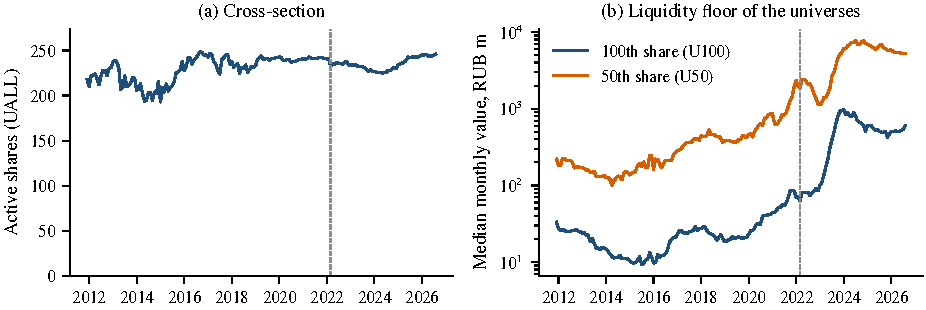
\includegraphics[width=\linewidth]{figures/fig_sample.pdf}
\caption{The cross-section of MOEX shares. Panel (a): number of active shares (UALL) at each formation month. Panel
(b): trailing 12-month median monthly trading value of the least liquid share in U100 and U50 (log scale, millions of
roubles). The dashed line marks the February 2022 suspension.}\label{fig:sample}
\end{figure}

% =====================================================================================
\section{Pre-specified research design}\label{sec:design}

\subsection{The pre-analysis plan}

The design was written down before estimation in a pre-analysis plan that fixes the sample, universes, the 25
characteristics with their windows, minimum data requirements and predicted signs, the portfolio rules, the test
statistics, the ladder of corrections, the robustness grid, the hypotheses and a list of commitments. Before the plan
was frozen, only diagnostics that do not condition on any characteristic had been examined: counts of shares,
sessions and dividends; the unconditional distribution of next-month returns in U100; the market-replication check
above; and the coverage of share counts. The plan was frozen on 10 October 2026 at 19:41 UTC; its SHA-256 hash and
those of the configuration and data-construction code were recorded and committed to a version-controlled repository
before the first characteristic was computed. This is an internal pre-specification rather than a filing with an
external registry, and it does not erase the author's knowledge of the published literature; its purpose is to make
every analytic choice visible and fixed in advance. Appendix~\ref{app:deviations} lists the deviations: a few
implementation details not spelled out in the plan, a bug fix found by an independent code audit after the results
were seen, a more efficient design of the power simulation, and several exploratory analyses added after seeing the
results, which are labelled as such wherever they appear.

\subsection{Characteristics}

Table~\ref{tab:defs} lists the 25 characteristics. They fall into seven clusters: momentum (12-1, 6-1 and 12-7 month
momentum, residual momentum and nearness to the 52-week high), reversal (one-month and long-term), seasonality, low
risk (Dimson beta, idiosyncratic and total volatility, maximum daily return), skewness and downside risk (downside
beta, total, idiosyncratic and co-skewness), size and liquidity (size, Amihud illiquidity, trading value, turnover,
the zero-return proportion, the Corwin--Schultz spread, the variability of trading value and abnormal trading volume)
and payout (dividend yield). Each is computed at the last session of month $t$ from data available at that time; the
exception is the fallback share counts behind size and turnover, which contain look-ahead and have a point-in-time
variant (Section~\ref{sec:universes}). Perturbation tests confirm that no characteristic, universe membership or cost
estimate changes when the price and trading data after $t$ are altered (Appendix~\ref{app:data}). The predicted sign is
the direction reported in the source paper (for the zero-return proportion and the spread, whose source papers propose
measures, in the paper that relates the measure to returns).

The implementations follow the sources where daily market data allow and adapt them where they do not, and all
portfolios follow the common protocol below whatever the holding rule of the source. Appendix
Table~\ref{tab:adapt} lists the differences. The substantive ones are four. Residual momentum and idiosyncratic
volatility use CAPM rather than Fama--French three-factor residuals, because without book equity there is no value
factor; Section~\ref{sec:robust} re-estimates both with a two-factor model that adds a size factor built from the
sample. Total skewness is measured from daily returns over a year rather than as the intraday realised skewness of
\citet{amaya2015realized}, and idiosyncratic skewness is historical rather than the model-based expected skewness of
\citet{boyer2010expected}. The beta portfolio is a low-minus-high quintile spread on \citet{dimson1979risk} betas
rather than the beta-neutral, leveraged portfolio of \citet{frazzini2014betting}, so its CAPM alpha is the closer test
of their prediction. Several windows and horizons also differ (coskewness from daily rather than monthly returns;
abnormal volume over a month rather than a day or a week; long-term reversal, seasonality and the variability of
trading value over shorter histories). A failure to survive is therefore a statement about the implemented signal,
not necessarily about the original anomaly.

\begin{table}[!htbp]
\centering\footnotesize
\caption{The 25 characteristics}\label{tab:defs}
\resizebox{\linewidth}{!}{\begin{tabular}{llp{6.3cm}cl}
\toprule
ID & Cluster & Definition (at the last session of month $t$) & Sign & Source \\
\midrule
MOM12\_1 & Momentum & $\prod_{j=1}^{11}(1+R_{t-j})-1$ & $+$ & \citet{jegadeesh1993returns} \\
MOM6\_1 & Momentum & $\prod_{j=1}^{5}(1+R_{t-j})-1$ & $+$ & \citet{jegadeesh1993returns} \\
MOM12\_7 & Momentum & $\prod_{j=6}^{11}(1+R_{t-j})-1$ & $+$ & \citet{novymarx2012momentum} \\
RESMOM & Momentum & CAPM residuals $t{-}11..t{-}1$ / their s.d.; betas from $t{-}35..t{-}1$ & $+$ & \citet{blitz2011residual} \\
HIGH52 & Momentum & $P_t / \max P$ over 252 sessions & $+$ & \citet{george2004week} \\
\addlinespace[2pt]
STR & Reversal & $R_t$ & $-$ & \citet{jegadeesh1990evidence} \\
LTR & Reversal & $\prod_{j=12}^{35}(1+R_{t-j})-1$ & $-$ & \citet{debondt1985overreact} \\
\addlinespace[2pt]
SEAS & Seasonality & mean of $R_{t+1-12j}$, $j=1..5$ & $+$ & \citet{heston2008seasonality} \\
\addlinespace[2pt]
BETA & Low risk & Dimson beta ($m_d$, $m_{d-1}$), 252 sessions & $-$ & \citet{frazzini2014betting} \\
IVOL & Low risk & s.d.\ of CAPM residuals, month $t$ & $-$ & \citet{ang2006cross} \\
TVOL & Low risk & s.d.\ of $r_d$, month $t$ & $-$ & \citet{ang2006cross} \\
MAX & Low risk & $\max r_d$, month $t$ & $-$ & \citet{bali2011maxing} \\
\addlinespace[2pt]
DBETA & Skewness/downside & beta on days with $m_d<\bar m$, 252 sessions & $+$ & \citet{ang2006downside} \\
SKEW & Skewness/downside & skewness of $r_d$, 252 sessions & $-$ & \citet{amaya2015realized} \\
ISKEW & Skewness/downside & skewness of CAPM residuals, 252 sessions & $-$ & \citet{boyer2010expected} \\
COSKEW & Skewness/downside & $E[\varepsilon_i\varepsilon_m^2]/(\sqrt{E\varepsilon_i^2}E\varepsilon_m^2)$, 252 sessions & $-$ & \citet{harvey2000conditional} \\
\addlinespace[2pt]
SIZE & Size/liquidity & $\log$ market cap$_t$ & $-$ & \citet{banz1981relationship} \\
AMIHUD & Size/liquidity & mean $|r_d|/\text{value}_d$, 252 sessions & $+$ & \citet{amihud2002illiquidity} \\
DVOL & Size/liquidity & $\log$ mean daily value, 252 sessions & $-$ & \citet{brennan1998alternative} \\
TURN & Size/liquidity & $\sum$ value$_{t-11..t}$ / mean cap & $-$ & \citet{datar1998liquidity} \\
ZERO & Size/liquidity & share of no-trade or zero-return sessions, 252 sessions & $+$ & \citet{lesmond1999new}; \citet{bekaert2007liquidity} \\
SPREAD & Size/liquidity & Corwin--Schultz spread, month $t$ & $+$ & \citet{corwin2012simple}; \citet{amihud1986asset} \\
CVVAL & Size/liquidity & s.d./mean of monthly value, $t{-}11..t$ & $-$ & \citet{chordia2001trading} \\
ABVOL & Size/liquidity & $\log$(daily value in $t$ / daily value $t{-}12..t{-}1$) & $+$ & \citet{gervais2001high} \\
\addlinespace[2pt]
DY & Payout & 12-month gross dividends / $P_t$ (payers only) & $+$ & \citet{litzenberger1979effect} \\
\bottomrule
\end{tabular}}
\tabnote{$R_t$: monthly total return; $r_d$: daily total return; $m_d$: daily MCFTRR return; ``252 sessions'' are the
252 sessions ending at the last session of month $t$; ``month $t$'' uses the sessions of the formation month. Minimum
data: all required months for momentum; at least 20 of 24 months for LTR; at least two years for SEAS; at least 24
months for RESMOM; 120 valid daily returns for the 12-month return-based measures, 120 trading days for HIGH52 and
DVOL, and 120 sessions since the first trade for ZERO; 15 valid daily returns for one-month measures; 12 valid two-day
pairs for SPREAD. Sign: the direction of predictability reported in the source; long--short portfolios are oriented
so that a positive mean confirms it. For ZERO and SPREAD the first source proposes the measure and the second relates
illiquidity of that kind to expected returns. DY is sorted among dividend payers only. Appendix Table~\ref{tab:adapt}
lists the differences from the source definitions.}
\end{table}

\subsection{Portfolios}

At the end of each month, the shares in the universe with a non-missing characteristic are sorted into quintiles,
ties broken by ticker; a factor-month requires at least 25 shares. Portfolios are equally weighted in the baseline,
and the long--short return is the top minus the bottom quintile, oriented by the predicted sign. Portfolios are held
for one month and rebalanced monthly; returns are gross of costs and taxes. Equal weights are natural here: U100
excludes the illiquid tail, and value weights in a market as concentrated as Russia's would make each quintile a bet on
a handful of firms. Capped value weights \citep{jensen2023replication} are a robustness variant.

\subsection{Test statistics and the ladder}

Let $r_{k,t}$ be the oriented long--short return of characteristic $k=1,\dots,K$ ($K=25$) in month $t$, with mean
$\bar r_k$ over its $n_k$ available months. The test statistic is $t_k=\bar r_k/\widehat{\mathrm{se}}(\bar r_k)$
with the \citet{newey1987simple} variance
\begin{equation}
\widehat{V}(\bar r_k)=\frac{1}{n_k^{2}}\Big[\sum_t e_{k,t}^2+2\sum_{j=1}^{L}\Big(1-\frac{j}{L+1}\Big)\sum_{t}e_{k,t}e_{k,t-j}\Big],
\qquad L=\lfloor 4(T/100)^{2/9}\rfloor=4,
\end{equation}
where $e_{k,t}=r_{k,t}-\bar r_k$ in available months and zero otherwise. The two-sided $p$-value is $p_k$. A
\emph{discovery} is a rejection with $t_k>0$; rejections with the opposite sign are reported separately. The ladder has
seven rungs:
\begin{enumerate}[label=R\arabic*.]
\item Conventional: $t_k>1.96$.
\item The \citet{harvey2016cross} hurdle: $t_k>3$.
\item \citet{holm1979simple}: with ordered $p_{(1)}\le\dots\le p_{(K)}$, reject $(1),\dots,(i)$ as long as
$p_{(j)}\le\alpha/(K-j+1)$ for all $j\le i$; this controls the family-wise error rate (FWER).
\item \citet{benjamini1995controlling}: reject the $i^\ast$ smallest $p$-values, $i^\ast=\max\{i:p_{(i)}\le i\alpha/K\}$;
false-discovery rate (FDR) control under independence or positive dependence.
\item \citet{benjamini2001control}: as R4 with $\alpha$ replaced by $\alpha/\sum_{i=1}^{K}i^{-1}$; FDR control under
arbitrary dependence.
\item \citet{romano2005stepwise} stepdown with the studentised statistics. Months are resampled jointly for all factors
with the stationary bootstrap of \citet{politis1994stationary} (mean block length six months, $B=10{,}000$), and the
centred statistics $t^\ast_{k,b}=(\bar r^\ast_{k,b}-\bar r_k)/\widehat{\mathrm{se}}^\ast_{k,b}$ are computed with the
same Newey--West estimator in every resample. Starting from all hypotheses, the critical value is the 95\% quantile of
$\max_{k\in A}|t^\ast_{k,b}|$ over the set $A$ of hypotheses not yet rejected; all $k\in A$ with $|t_k|$ above it are
rejected and the step is repeated. Adjusted $p$-values follow \citet{romano2016efficient}. This rung controls the FWER
asymptotically while accounting for the dependence and the non-normality of the factor returns;
Section~\ref{sec:multiplicity} examines its size at the present sample length.
\item The Deflated Sharpe Ratio of \citet{bailey2014deflated}. With monthly Sharpe ratio $\widehat{SR}_k$, skewness
$\hat\gamma_{3,k}$ and kurtosis $\hat\gamma_{4,k}$,
\begin{equation}
\mathrm{DSR}_k=\Phi\!\left(\frac{(\widehat{SR}_k-SR_0)\sqrt{n_k-1}}{\sqrt{1-\hat\gamma_{3,k}\widehat{SR}_k+\frac{\hat\gamma_{4,k}-1}{4}\widehat{SR}_k^2}}\right),\quad
SR_0=\sqrt{\widehat V[\widehat{SR}]}\Big[(1-\gamma)\Phi^{-1}\Big(1-\tfrac{1}{N}\Big)+\gamma\Phi^{-1}\Big(1-\tfrac{1}{Ne}\Big)\Big],
\end{equation}
where $\gamma$ is the Euler--Mascheroni constant, $N=25$ and $\widehat V[\widehat{SR}]$ is the cross-sectional variance
of the 25 Sharpe ratios. A factor passes if $\mathrm{DSR}_k>0.95$.
\end{enumerate}
At the level of the family I report the probability of backtest overfitting (PBO) of choosing the in-sample best of the
25 factors, estimated by combinatorially symmetric cross-validation with 16 blocks \citep{bailey2017probability}, and
the effective number of independent tests from the eigenvalues $\lambda_i$ of the factor correlation matrix, both as
$1+(K-1)(1-\mathrm{Var}(\lambda)/K)$ \citep{nyholt2004simple} and as $\sum_i[\mathbb 1(\lambda_i\ge1)+(\lambda_i-\lfloor\lambda_i\rfloor)]$
\citep{li2005adjusting}.

\paragraph{An empirical-Bayes complement.}
Frequentist corrections ask which individual factors can be declared real while controlling the error rate across the
family. \citet{jensen2023replication} ask instead what can be inferred about each factor's premium when the premia are
themselves drawn from a common distribution. Following them, let $\hat{\boldsymbol\mu}=\boldsymbol\mu+\boldsymbol\varepsilon$,
$\boldsymbol\varepsilon\sim N(0,\Sigma)$, where $\Sigma$ is the sample covariance of the factor returns divided by the
sample length, and $\mu_k=\mu_0+c_{j(k)}+w_k$ with cluster effects $c_j\sim N(0,\tau_c^2)$ for the seven clusters of
Table~\ref{tab:defs} (Appendix~\ref{app:deviations} discusses the nine labels used in one table of the plan) and
idiosyncratic effects $w_k\sim N(0,\tau_w^2)$. The hyperparameters are estimated by maximum
marginal likelihood; the posterior of $\boldsymbol\mu$ is normal, and a factor ``replicates'' if its 95\% posterior
interval excludes zero on the positive side.

\subsection{Hypotheses}

The plan states five hypotheses. H1: each oriented premium is positive ($\mu_k>0$), evaluated under every rung. H2:
the global null that all $\mu_k=0$, tested with the single-step max-$|t|$ bootstrap. H3: the number of discoveries does
not increase along the ladder (descriptive). H4: premia differ between the periods before and after March 2022, for
each factor and for the average of the 25---exploratory, given a post-break sample of 55 months. H5: factors that
survive the \RW{} rung earn positive returns net of estimated trading costs.

The robustness grid comprises capped value weights, U50, UALL, terciles, a one-session implementation lag (entry at the
close of the first trade in month $t+1$), U100 without preferred shares whose ordinary share is also in U100,
price-only holding returns, the exclusion of the transition months February and March 2022, CAPM alphas, and
point-in-time size and turnover. Every variant is run through the full ladder; the \RW{} test is also repeated with
mean block lengths of three and twelve months. For the DSR sensitivity the plan sets $N=250$, its count of
configurations in the grid.

% =====================================================================================
\section{Results}\label{sec:results}

\subsection{Single-test evidence}

Table~\ref{tab:baseline} reports the baseline long--short portfolios and Figure~\ref{fig:ladder} shows their
$t$-statistics against the thresholds of the ladder. The momentum cluster dominates. Nearness to the 52-week high
earns \val{MeanHIGH52}\% a month ($t=\val{THIGH52}$, annualised Sharpe ratio \val{SRHIGH52}); six-month momentum
\val{MeanMOM61}\% ($t=\val{TMOM61}$); residual momentum \val{MeanRESMOM}\% ($t=\val{TRESMOM}$); twelve-month momentum
\val{MeanMOM121}\% ($t=\val{TMOM121}$); and twelve-to-seven-month momentum \val{MeanMOM127}\% ($t=\val{TMOM127}$). Two
trading-activity characteristics also clear the conventional bar: abnormal trading volume (\val{MeanABVOL}\%,
$t=\val{TABVOL}$) and the variability of trading value (\val{MeanCVVAL}\%, $t=\val{TCVVAL}$). CAPM alphas are close to
the raw means because the average market excess return over the sample was small (\val{MktExcess}\% a month).

Nothing else clears $t>1.96$ in the predicted direction. Low-risk portfolios have positive but insignificant means
(beta, $t=\val{TBETA}$; idiosyncratic volatility, $t=\val{TIVOL}$; maximum return, $t=\val{TMAX}$). Size
($t=\val{TSIZE}$), Amihud illiquidity ($t=\val{TAMIHUD}$), the zero-return proportion ($t=\val{TZERO}$), dividend yield
($t=\val{TDY}$), seasonality ($t=\val{TSEAS}$) and long-term reversal ($t=\val{TLTR}$) are statistically zero, and the
spread portfolio has the wrong sign ($t=\val{TSPREAD}$). The most striking failure is the one-month reversal: the
portfolio that buys last month's losers and sells last month's winners loses \val{MeanAbsSTR}\% a month
($t=\val{TSTR}$). Section~\ref{sec:str} returns to this short-term continuation.

\begin{table}[!htbp]
\centering\small
\caption{Baseline long--short portfolios and the ladder of significance}\label{tab:baseline}
\resizebox{\linewidth}{!}{\begin{tabular}{lrrrrrrr ccccccc r}
\toprule
 & \multicolumn{7}{c}{Long--short return (predicted direction)} & \multicolumn{7}{c}{Discovery under rung} & \\
\cmidrule(lr){2-8}\cmidrule(lr){9-15}
Factor & Mean & $t$ & SR & $\alpha$ & $t(\alpha)$ & $\beta$ & Skew & R1 & R2 & R3 & R4 & R5 & R6 & R7 & $p_{\text{RW}}$ \\
\midrule
MOM12\_1 & 2.28 & 4.72 & 1.17 & 2.31 & 4.98 & $-$0.36 & $-$2.08 & \checkmark & \checkmark & \checkmark & \checkmark & \checkmark & \checkmark &  & 0.002 \\
MOM6\_1 & 2.19 & 5.33 & 1.34 & 2.22 & 5.62 & $-$0.31 & $-$0.43 & \checkmark & \checkmark & \checkmark & \checkmark & \checkmark & \checkmark &  & 0.001 \\
MOM12\_7 & 1.54 & 3.24 & 0.84 & 1.57 & 3.46 & $-$0.35 & $-$1.66 & \checkmark & \checkmark & \checkmark & \checkmark & \checkmark &  &  & 0.058 \\
RESMOM & 1.64 & 4.90 & 1.28 & 1.66 & 5.01 & $-$0.15 & $-$0.43 & \checkmark & \checkmark & \checkmark & \checkmark & \checkmark & \checkmark &  & 0.001 \\
HIGH52 & 3.08 & 6.07 & 1.44 & 3.13 & 5.95 & $-$0.43 & $-$1.44 & \checkmark & \checkmark & \checkmark & \checkmark & \checkmark & \checkmark &  & 0.000 \\
\addlinespace[2pt]
STR & $-$1.96 & $-$4.96 & $-$1.23 & $-$1.98 & $-$4.76 & 0.18 & 0.12 & $\times$ &  &  &  &  & $\times$ &  & 0.001 \\
LTR & 0.08 & 0.19 & 0.05 & 0.07 & 0.16 & 0.14 & 2.13 &  &  &  &  &  &  &  & 0.999 \\
\addlinespace[2pt]
SEAS & $-$0.12 & $-$0.41 & $-$0.10 & $-$0.11 & $-$0.40 & $-$0.09 & $-$0.66 &  &  &  &  &  &  &  & 0.999 \\
\addlinespace[2pt]
BETA & 0.69 & 1.52 & 0.37 & 0.75 & 1.74 & $-$0.58 & $-$0.87 &  &  &  &  &  &  &  & 0.773 \\
IVOL & 0.85 & 1.85 & 0.48 & 0.91 & 2.18 & $-$0.35 & $-$1.29 &  &  &  &  &  &  &  & 0.575 \\
TVOL & 0.72 & 1.46 & 0.39 & 0.80 & 1.87 & $-$0.49 & $-$1.20 &  &  &  &  &  &  &  & 0.787 \\
MAX & 0.06 & 0.13 & 0.04 & 0.12 & 0.27 & $-$0.33 & $-$1.53 &  &  &  &  &  &  &  & 0.999 \\
\addlinespace[2pt]
DBETA & $-$0.35 & $-$0.89 & $-$0.22 & $-$0.40 & $-$1.04 & 0.48 & 0.80 &  &  &  &  &  &  &  & 0.984 \\
SKEW & 0.56 & 1.46 & 0.38 & 0.56 & 1.47 & $-$0.02 & $-$0.54 &  &  &  &  &  &  &  & 0.787 \\
ISKEW & 0.24 & 0.59 & 0.16 & 0.24 & 0.62 & $-$0.07 & $-$0.48 &  &  &  &  &  &  &  & 0.996 \\
COSKEW & 0.06 & 0.21 & 0.06 & 0.05 & 0.18 & 0.10 & $-$0.41 &  &  &  &  &  &  &  & 0.999 \\
\addlinespace[2pt]
SIZE & 0.18 & 0.41 & 0.13 & 0.18 & 0.40 & 0.03 & 0.04 &  &  &  &  &  &  &  & 0.999 \\
AMIHUD & $-$0.16 & $-$0.39 & $-$0.09 & $-$0.14 & $-$0.37 & $-$0.13 & 1.23 &  &  &  &  &  &  &  & 0.999 \\
DVOL & 0.24 & 0.70 & 0.16 & 0.26 & 0.81 & $-$0.19 & 0.95 &  &  &  &  &  &  &  & 0.995 \\
TURN & 0.62 & 1.52 & 0.46 & 0.66 & 1.93 & $-$0.37 & $-$0.44 &  &  &  &  &  &  &  & 0.773 \\
ZERO & $-$0.32 & $-$0.70 & $-$0.20 & $-$0.30 & $-$0.68 & $-$0.16 & 0.73 &  &  &  &  &  &  &  & 0.995 \\
SPREAD & $-$0.83 & $-$1.74 & $-$0.42 & $-$0.90 & $-$2.01 & 0.40 & 1.48 &  &  &  &  &  &  &  & 0.644 \\
CVVAL & 0.98 & 2.79 & 0.63 & 0.97 & 2.81 & 0.04 & $-$1.36 & \checkmark &  &  & \checkmark &  &  &  & 0.137 \\
ABVOL & 1.40 & 3.52 & 1.02 & 1.38 & 3.75 & 0.20 & 0.23 & \checkmark & \checkmark & \checkmark & \checkmark & \checkmark & \checkmark &  & 0.033 \\
\addlinespace[2pt]
DY & 0.16 & 0.37 & 0.12 & 0.17 & 0.44 & $-$0.21 & $-$0.17 &  &  &  &  &  &  &  & 0.999 \\
\midrule
\multicolumn{8}{l}{Number of discoveries (of 25)} & 7 & 6 & 6 & 7 & 6 & 5 & 0 & \\
\bottomrule
\end{tabular}}
\tabnote{Equal-weighted quintile long--short portfolios in U100, oriented by the predicted sign (Table~\ref{tab:defs}).
Mean and $\alpha$ in \% per month; $t$-statistics with Newey--West standard errors ($L=4$). SR: annualised Sharpe ratio.
$\alpha$, $\beta$: intercept and slope of the regression on the MCFTRR excess return. Rungs: R1 $t>1.96$; R2 $t>3$;
R3 Holm; R4 Benjamini--Hochberg; R5 Benjamini--Yekutieli; R6 \RW{} stepdown (stationary bootstrap, mean block 6,
$B=10{,}000$); R7 Deflated Sharpe Ratio $>0.95$ with $N=25$. \cmark: discovery in the predicted direction; $\times$:
significant with the opposite sign. $p_{\text{RW}}$: \RW{} adjusted $p$-value. Holding months 2012:01--2026:09
($T=177$). IVOL, TVOL, MAX and SPREAD have 176 months because March 2022 had only six sessions, too few for the
one-month daily measures; DY has 176 because fewer than 25 U100 shares had a trailing dividend in May 2014
(Section~\ref{sec:returns}).}
\end{table}

\begin{figure}[!htbp]
\centering
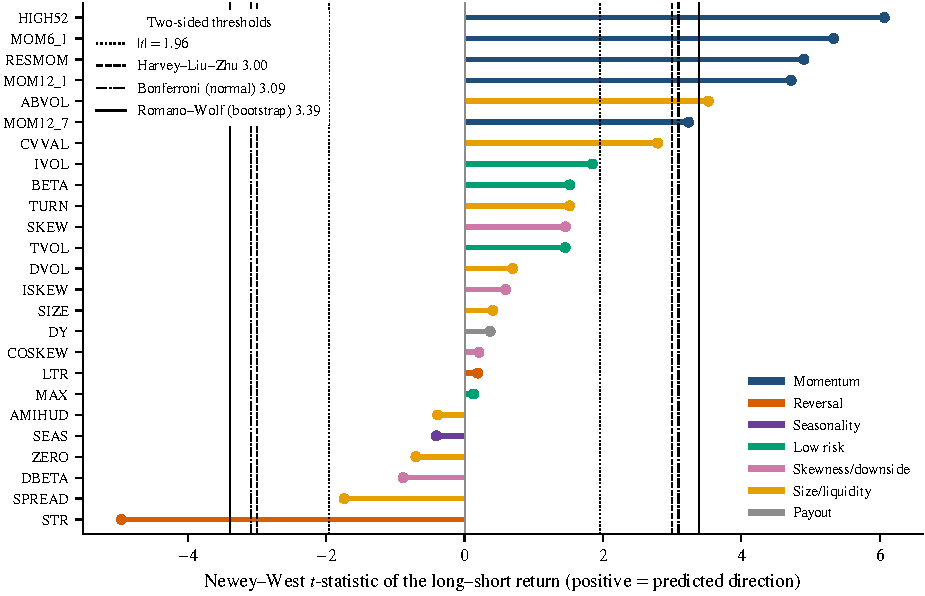
\includegraphics[width=\linewidth]{figures/fig_ladder.pdf}
\caption{The factor zoo on MOEX. Newey--West $t$-statistics of the 25 oriented long--short portfolios (baseline),
coloured by cluster, against the conventional, Harvey--Liu--Zhu, normal-theory Bonferroni and \RW{} (first-step,
bootstrap) thresholds.}\label{fig:ladder}
\end{figure}

\subsection{Correcting for multiplicity}\label{sec:multiplicity}

The global null that no characteristic predicts returns is rejected decisively: the largest $|t|$ is far beyond the
bootstrap distribution of the maximum ($p=\val{GlobalNullP}$), confirming H2. The bottom row of
Table~\ref{tab:baseline} and the first row of Table~\ref{tab:counts} show how the discoveries thin out along the
ladder: seven at R1, six at R2, six under Holm, seven under Benjamini--Hochberg, six under Benjamini--Yekutieli, five
under \RW{} and none under the Deflated Sharpe Ratio. The five \RW{} survivors are the 52-week high, six-month momentum,
residual momentum, twelve-month momentum and abnormal volume. Twelve-to-seven-month momentum clears the Harvey--Liu--Zhu,
Holm and Benjamini--Hochberg bars but not \RW{} ($p_{\text{RW}}=\val{PrwMOM127}$); the variability of trading value
clears only R1 and Benjamini--Hochberg.

The \RW{} critical value deserves attention. At the first step it equals \val{RWcrit}, more than the Harvey--Liu--Zhu
hurdle and more than \val{BonfCrit}, the Bonferroni bound for 25 two-sided normal tests. Three forces determine it,
and simulations separate them (Figure~\ref{fig:boot}). Dependence among the factors lowers the bar: the factors are
correlated (the mean absolute pairwise correlation is \val{MeanAbsCorr}, and the first eigenvalue of their correlation
matrix is \val{EigOne}, or \val{EigShare}\% of the total), and standard normal statistics with the factors' correlation
matrix have a 95\% quantile of the maximum of \val{QnormCorr} instead of \val{QnormIndep} for independent ones. The
reduction is smaller than the eigenvalue-based effective number of tests suggests (\val{NeffLiJi} by the Li--Ji formula
and \val{NeffNyholt} by Nyholt's; \val{NeffLiJi} independent tests would give \val{MechSidakNeff}), because moderate
correlations matter little in the extreme tail that a family-wise test controls. Estimation noise in the Newey--West
standard error raises the bar: with 177 monthly observations the studentised statistics are more dispersed than
$N(0,1)$. For i.i.d.\ normal returns a Newey--West $t$-statistic with $L=4$ exceeds 3.09 in absolute value with
probability \val{MechIidPthree} rather than 0.0020, and with the factors' correlation matrix the 95\% quantile of the
maximum rises to \val{QiidCorrL4}. The remaining \val{DecompData} reflects features of the actual returns that the
bootstrap preserves and the i.i.d.\ benchmark does not, such as serial dependence and volatility clustering;
consistent with this, the critical value rises with the bootstrap block length, to \val{RWcritB3}, \val{RWcrit} and
\val{RWcritB12} for mean blocks of three, six and twelve months.

Fat tails of the returns are not responsible:
replacing every factor's returns by the normal scores of their ranks, which sets the kurtosis to three while keeping the
dependence, raises the critical value slightly, to \val{MechNormalScores}. In the bootstrap the centred statistics have
a median standard deviation of \val{MechSDmed} (between \val{MechSDmin} and \val{MechSDmax} across factors) but nearly
normal tails (median kurtosis \val{MechKurtMed}); rescaling them to unit variance lowers the critical value to
\val{MechRescaled}, so most of the excess comes from their dispersion rather than their shape. A longer HAC lag does not help, because
it makes the variance estimate noisier: the critical value rises to \val{MechCritLeight} with $L=8$ and
\val{MechCritLtwelve} with $L=12$, roughly in step with the i.i.d.\ benchmark (\val{QiidCorrL8} and \val{QiidCorrL12}). Procedures that convert $t$-statistics into normal $p$-values---Holm and both FDR rules---therefore understate
the multiplicity burden in samples of this length, and the rule of thumb $t>3$ is not conservative enough. The noise in
the variance estimate is generic to any fifteen-year monthly sample, the typical history of an emerging market; the
other two components depend on the data. The survivors are the same with mean blocks of three and twelve months except that
twelve-to-seven-month momentum enters with the shorter block and abnormal volume drops out with the longer one. Monte
Carlo error is modest: with five other seeds the first-step critical value lies between \val{SeedCritMin} and
\val{SeedCritMax} and the survivors are \val{SeedSame}, with abnormal volume a marginal case (adjusted $p$ between
\val{SeedPabvolMin} and \val{SeedPabvolMax}).

The \RW{} guarantee is asymptotic, and at this sample length the test is mildly liberal. In \val{FWreps} simulated
samples under the global null in each of two designs (Appendix~\ref{app:data}; exploratory), it commits a family-wise
error in \val{FWrwPar}\% (95\% interval \val{FWrwParLo}--\val{FWrwParHi}\%) and \val{FWrwBoot}\%
(\val{FWrwBootLo}--\val{FWrwBootHi}\%) of the samples, against a nominal 5\%. The normal-theory procedures err more
often: Holm, which under the global null rejects exactly when Bonferroni does, in \val{FWholmPar}\% and
\val{FWholmBoot}\% of the samples, and the $t>3$ rule in \val{FWtthreePar}\% and \val{FWtthreeBoot}\%. Calibrating the
nominal level so that the simulated error rate does not exceed 5\% in either design gives $\alpha^\ast=\val{FWalphaStar}$
and a first-step critical value of \val{FWcritStar}. At that level the four momentum survivors and the wrong-signed
short-term reversal remain significant, while abnormal volume (adjusted $p=\val{FWpAbvol}$) does not
(Table~\ref{tab:revchecks}).

\begin{figure}[!htbp]
\centering
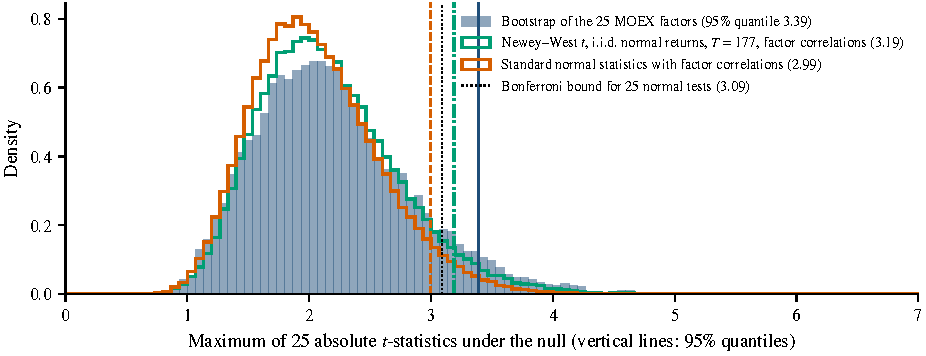
\includegraphics[width=\linewidth]{figures/fig_boot.pdf}
\caption{Distribution of the maximum of 25 absolute $t$-statistics under the null: stationary bootstrap of the 25 MOEX
factors (mean block 6, $B=10{,}000$); Newey--West $t$-statistics ($L=4$) computed from i.i.d.\ normal returns with
$T=177$ and the factors' correlation matrix (100{,}000 replications); and standard normal statistics with the same
correlation matrix. Vertical lines mark the 95\% quantiles; the dotted line is the Bonferroni bound for 25 independent
normal tests.}\label{fig:boot}
\end{figure}

No factor passes the pre-specified Deflated Sharpe Ratio. The reason is the benchmark. With $N=25$ the expected maximum
Sharpe ratio under the null is computed from the cross-sectional variance of the 25 estimated Sharpe ratios, and that
variance contains the true dispersion between strong momentum factors and a strongly negative short-term reversal, not
only estimation noise. The implied benchmark is an annualised Sharpe ratio of \val{SRzeroN}, so even the best factor,
with \val{SRHIGH52}, has a DSR of only \val{DsrHIGH52}. Using the effective number of tests ($N=\val{NeffLiJi}$) lowers
the benchmark to \val{SRzeroNeff} and changes nothing; using the 250 configurations of the robustness grid raises it to
\val{SRzeroAll}. As an exploratory diagnostic I replace the benchmark by the expected maximum Sharpe ratio under the
dependence-preserving bootstrap null. The benchmark falls to \val{SRzeroBoot}, and exactly the five \RW{} survivors pass.
The closed-form DSR is a useful screen for a researcher's own specification search, where the trials are variations of one
strategy; applied to a zoo of genuinely different factors, its variance-based benchmark is extremely conservative.

At the family level, the probability that the in-sample best of the 25 factors underperforms the median factor out of
sample is \val{PBO} (CSCV on the \val{PBOT} months in which all factors are available). The in-sample winner is a momentum
variant in \val{PBOmom}\% of the 12{,}870 splits (the 52-week high alone in \val{PBOhigh}\%) and abnormal volume in
\val{PBOabvol}\%; out of sample it ranks among the top five of the 25 factors in \val{PBOtopfive}\% of splits, and its
median rank is \val{PBOrankWord}. Read literally, H3 fails at one step: Benjamini--Hochberg, which controls the false-discovery
rather than the family-wise error rate, admits one factor more than Holm (the variability of trading value). The count
never exceeds its conventional level; it falls from seven to six at the Harvey--Liu--Zhu, Holm and
Benjamini--Yekutieli rungs, which drop the variability of trading value, and to five at the \RW{} rung, which also drops
twelve-to-seven-month momentum.

\begin{table}[!htbp]
\centering\small
\caption{Number of discoveries along the ladder, all specifications}\label{tab:counts}
\begin{tabular}{l ccccccc cc}
\toprule
Specification & R1 & R2 & R3 & R4 & R5 & R6 & R7 & Wrong sign & RW crit. \\
 & $t{>}1.96$ & $t{>}3$ & Holm & BH & BY & RW & DSR & (RW) & (step 1) \\
\midrule
Baseline (U100, EW, quintiles) & 7 & 6 & 6 & 7 & 6 & 5 & 0 & 1 & 3.39 \\
\quad RW mean block = 3 & 7 & 6 & 6 & 7 & 6 & 6 & 0 & 1 & 3.31 \\
\quad RW mean block = 12 & 7 & 6 & 6 & 7 & 6 & 4 & 0 & 1 & 3.55 \\
\addlinespace[2pt]
Capped value weights & 6 & 4 & 4 & 6 & 4 & 4 & 0 & 0 & 3.44 \\
U50 (50 most liquid) & 6 & 3 & 3 & 6 & 3 & 3 & 0 & 0 & 3.31 \\
UALL (all active shares) & 10 & 4 & 4 & 8 & 4 & 1 & 0 & 0 & 3.64 \\
Terciles & 7 & 6 & 6 & 6 & 6 & 6 & 0 & 1 & 3.36 \\
One-session implementation lag & 8 & 6 & 6 & 6 & 6 & 4 & 0 & 1 & 3.32 \\
Preferred duplicates dropped & 7 & 6 & 6 & 7 & 6 & 6 & 0 & 1 & 3.41 \\
Price-only holding returns & 7 & 4 & 4 & 5 & 4 & 4 & 0 & 1 & 3.36 \\
Excluding 2022-02, 2022-03 & 7 & 7 & 7 & 7 & 7 & 6 & 0 & 1 & 3.36 \\
Point-in-time SIZE/TURN & 7 & 6 & 6 & 7 & 6 & 5 & 0 & 1 & 3.42 \\
\addlinespace[2pt]
CAPM alpha (market-hedged) & 8 & 6 & 6 & 7 & 6 & 6 & 0 & 1 & 3.39 \\
Net of trading costs & 5 & 4 & 4 & 4 & 4 & 4 & 0 & 3 & 3.39 \\
\addlinespace[2pt]
Pre-2022 (2012-01--2022-02) & 7 & 5 & 5 & 6 & 6 & 4 & 0 & 1 & 3.47 \\
Post-2022 (2022-03--2026-09) & 8 & 1 & 1 & 1 & 1 & 0 & 0 & 0 & 3.93 \\
\bottomrule
\end{tabular}
\tabnote{Number of the 25 characteristics declared a discovery in the predicted direction under each rung. Wrong sign
(RW): \RW{} rejections with a negative oriented mean. RW crit.: first-step \RW{} critical value. Variants as described in
Section~\ref{sec:design}. CAPM alpha: ladder applied to market-hedged returns. Net of trading costs: returns after the
cost model of Section~\ref{sec:costs}. Pre/post-2022: ladders estimated separately in each regime (exploratory).}
\end{table}

\subsection{Short-term continuation}\label{sec:str}

The one-month reversal is one of the oldest anomalies \citep{jegadeesh1990evidence}. On MOEX it has the wrong sign: in
U100 the winners of month $t$ beat its losers by \val{MeanAbsSTR}\% in month $t+1$, a \RW{}-significant rejection of
the reversal hypothesis in the opposite direction. The continuation is unlikely to be a microstructure artefact. Bid--ask
bounce and stale prices would produce reversal, not continuation, and the effect is even stronger when the portfolio is entered
at the close of the first trade of the holding month ($t=-5.46$; Table~\ref{tab:robust_t}). It is present before and
after 2022 ($t=\val{RegTpreSTR}$ and $\val{RegTpostSTR}$), in U50 ($t=-3.27$) and with value weights ($t=-2.40$), and it
survives a Fama--MacBeth control for twelve-month momentum (Section~\ref{sec:fm}). It disappears, however, in the broad universe UALL ($t=0.29$),
which adds the least liquid shares.

\citet{medhat2022short} show that the one-month reversal in the United States is confined to low-turnover stocks,
while high-turnover stocks display short-term momentum. In an exploratory analysis (Table~\ref{tab:str}, panel A) I sort
UALL into turnover terciles and, within each, form quintiles on the past month's return. Among low-turnover shares last
month's winners underperform ($\val{STRlowM}$\%, $t=\val{STRlowT}$), among high-turnover shares they outperform
(\val{STRhighM}\%, $t=\val{STRhighT}$), and the difference, \val{STRdiffM}\% a month, is significant
($t=\val{STRdiffT}$), although neither tercile is significant on its own. Turnover does not explain the continuation in
U100, however. Only about half of U100 shares (\val{UhundTopTurn}\%) belong to the top turnover tercile of UALL, and
within U100 continuation is strong in both the low-turnover half (\val{UhundLowTurnM}\%, $t=\val{UhundLowTurnT}$) and
the high-turnover half (\val{UhundHighTurnM}\%, $t=\val{UhundHighTurnT}$), with an insignificant difference
($t=\val{UhundDiffT}$; panel B). Continuation is thus a property of the liquid segment as a whole, and weak signs of
the usual reversal appear only in the lowest turnover tercile of the broad cross-section. A continuation strategy in U100 turns over
\val{ContTurnover} times its notional a month; net of the cost model of Section~\ref{sec:costs} it would still earn
about \val{ContNetMean}\% a month ($t=\val{ContNetT}$) before price impact, which on the illustrative calculation of
Section~\ref{sec:costs} would eliminate it at any meaningful size---a borderline and post hoc result.

\begin{table}[!htbp]
\centering\small
\caption{Short-term returns by turnover (exploratory)}\label{tab:str}
\begin{tabular}{lrr}
\toprule
 & Winners $-$ losers of month $t$ & $t$ \\
\midrule
\multicolumn{3}{l}{\textit{A. All active shares (UALL), turnover terciles}} \\
\quad Low turnover & $-$1.23 & $-$1.90 \\
\quad Medium turnover & $-$0.24 & $-$0.38 \\
\quad High turnover & 1.04 & 1.58 \\
\quad High $-$ low & 2.28 & 2.84 \\
\addlinespace[3pt]
\multicolumn{3}{l}{\textit{B. Liquid universe (U100), turnover halves}} \\
\quad Low turnover & 1.38 & 3.16 \\
\quad High turnover & 1.96 & 3.54 \\
\quad High $-$ low & 0.58 & 1.15 \\
\bottomrule
\end{tabular}
\tabnote{Panel A: within UALL, shares are sorted each month into terciles of turnover (TURN) and, within each tercile,
into quintiles of the month-$t$ return. Panel B: the same within U100, with turnover halves. The table reports the mean
return in month $t+1$ of the top minus the bottom quintile (winners minus losers, \% per month) with Newey--West
$t$-statistics. Positive values indicate continuation. Not part of the pre-analysis plan.}
\end{table}

\subsection{A Bayesian complement}\label{sec:eb}

The empirical-Bayes model gives a much more permissive answer. The estimated prior has mean \val{EBmuzero}\% a month,
a cluster dispersion $\tau_c=\val{EBtauc}$\% and an idiosyncratic dispersion of only $\tau_w=\val{EBtauw}$\%
(Appendix Table~\ref{tab:eb}, Figure~\ref{fig:eb}). Thirteen of the 25 posterior intervals exclude zero on the positive
side, a ``replication rate'' of \val{EBrate}\%. The composition of that set is revealing: it consists of every member of
the momentum cluster and every member of the size-and-liquidity cluster, including the Amihud, zero-return and spread
portfolios whose own means are negative. With $\tau_w$ close to zero the model pools almost completely within clusters,
so the posterior answers whether the average premium of a theme is positive---for liquidity it is, because abnormal
volume and the variability of trading value pull the cluster mean up---rather than whether a particular characteristic
predicts returns. With the nine cluster labels used in one table of the plan, which separate downside risk from
skewness and size from liquidity, the replicated set is \val{EBnineSame}. Without clusters (exploratory) the model
declares \val{EBncPos} factors replicated, but a different set: it includes six portfolios whose own $t$-statistics are
below 1.9 (idiosyncratic and total volatility, skewness, size, trading value and turnover) and excludes
twelve-to-seven-month momentum ($t=\val{TMOM127}$); it ranks the 52-week high below skewness and shrinks the short-term
reversal, with its $t$-statistic of $\val{TSTR}$, to a posterior mean close to zero. These results reflect strong
shrinkage across factors whose estimation errors are almost collinear (the correlation is \val{CorrIvolTvol} between the
idiosyncratic- and total-volatility portfolios and \val{CorrMomMom} between twelve-month and twelve-to-seven-month
momentum). In both versions the posterior standard deviations (median \val{EBpostSDmed}\% with clusters) are well below
the sampling standard errors of the means (median \val{OLSseMed}\%), as shrinkage implies, but because the
hyperparameters are estimated from only 25 premia and then treated as known, these intervals understate the
uncertainty. The Bayesian replication rate is therefore fragile in this setting, and it answers a different
question from the frequentist ladder. For the question this paper asks---which specific predictors can be relied on in
Russia---the dependence-robust frequentist rung is the more informative.

\subsection{Robustness}\label{sec:robust}

Table~\ref{tab:counts} reports the ladder for every specification in the grid, and Appendix Table~\ref{tab:robust_t}
the $t$-statistics. The survivors are remarkably stable. Residual momentum survives \RW{} in every full-sample specification
of Table~\ref{tab:counts}, including UALL; twelve-month momentum and the 52-week high in all except UALL; six-month
momentum in all except value weights, U50 and UALL. Twelve-to-seven-month momentum survives with terciles, without
preferred duplicates, for CAPM alphas and with the shortest bootstrap block. Abnormal volume, by contrast, is fragile: it fails in U50, in UALL, with the
implementation lag, with price-only returns and with the longest bootstrap block. The failures with the implementation lag and with price-only returns suggest that part of its premium accrues at the very
start of the holding month and part through dividends; I do not pursue this further. The variability of trading value survives only when the 2022 transition
months are dropped.

In UALL, which adds about 130 less liquid shares, the conventional rung admits ten characteristics---among them
size ($t=2.45$), trading value ($t=3.11$), the zero-return proportion ($t=2.47$) and Amihud illiquidity
($t=2.00$), so the classic small-and-illiquid premia appear once the least liquid shares are included---but the
\RW{} critical value rises to 3.64 and only residual momentum survives: the illiquid tail adds noise faster than it
adds signal. With value weights and in U50 the momentum core survives, although with fewer variants. Dropping the
look-ahead in share counts leaves size and turnover insignificant. Excluding February and March 2022, the most extreme
months of the sample, raises rather than lowers the count.

\paragraph{Additional checks (exploratory).} Table~\ref{tab:revchecks} collects checks added after the first version of
the paper, each run through the full ladder. Unobserved delisting losses do not create the momentum premia. Many
terminal events are share exchanges or buyouts rather than losses, so a uniform delisting return is a stress test
rather than an estimate. Charging $-30$\%, the value used for performance-related delistings in US data since
\citet{shumway1997delisting}, $-50$\%, close to the $-55$\% that \citet{shumway1999delisting} estimate for Nasdaq, or
$-100$\% once to every terminal event leaves the momentum core and abnormal volume significant. In
\val{TermShortMoreWord} of the four momentum portfolios terminal events fall more often in the short leg (in the
52-week-high portfolio, \val{TermHIGHlong} in the long and \val{TermHIGHshort} in the short leg), so assumed losses tend
to raise their premia; residual momentum is the exception (\val{TermRESMOMlong} and \val{TermRESMOMshort}). The same
holds more strongly for the variability of trading value, whose short leg contains \val{TermCVVALshort} of its
\val{TermCVVALtot} terminal events; with losses of 100\% it also survives. A one-sided bound that charges $-100$\% to
every terminal event in a long leg and nothing to those in a short leg, and a two-sided bound that adds a 50\% buyout
premium to the events in short legs, keep all four momentum survivors, although in the two-sided case residual
momentum only just clears the bar ($t=\val{AdvTwoTRESMOM}$ against a critical value of \val{AdvTwoCrit}); abnormal
volume falls to $t=\val{AdvTABVOL}$ and $t=\val{AdvTwoTABVOL}$. Holding suspended shares until trading resumes changes
nothing. In 2013 the price source takes the volumes of some large shares from a thinly traded board; setting their
volume-based characteristics to missing for the affected months lowers the $t$-statistic of abnormal volume to
\val{BoardTABVOL} and leaves the survivors unchanged (Appendix~\ref{app:data}). Removing the six depositary-receipt histories (up to
\val{DRmaxWord} U100 shares a month from 2020) leaves the same five survivors. Re-estimating residual momentum and
idiosyncratic volatility with a two-factor model---the market and a value-weighted small-minus-big factor built from
all active shares, which inherits the look-ahead in share counts noted in Section~\ref{sec:data}---lowers the $t$-statistic of residual momentum from \val{TRESMOM} to \val{TwoFtRESMOM} and moves that
of idiosyncratic volatility from \val{TIVOL} to \val{TwoFtIVOL}; the survivors are unchanged. Book equity, and hence
a value factor, is not available.

\begin{table}[!htbp]
\centering\small
\caption{Additional checks (exploratory)}\label{tab:revchecks}
\resizebox{\linewidth}{!}{\begin{tabular}{l r rrrrr r l}
\toprule
 & RW & \multicolumn{5}{c}{$t$-statistic} & & \\
\cmidrule(lr){3-7}
Specification & crit. & HIGH52 & MOM6\_1 & RESMOM & MOM12\_1 & ABVOL & RW & Other \\
\midrule
Baseline & 3.39 & 6.07 & 5.33 & 4.90 & 4.72 & 3.52 & 5 & -- \\
\addlinespace[2pt]\multicolumn{9}{l}{\emph{Terminal events and suspensions}} \\
Delisting return $-30$\% & 3.38 & 6.14 & 5.27 & 4.71 & 4.75 & 3.72 & 5 & -- \\
Delisting return $-50$\% & 3.37 & 6.17 & 5.21 & 4.56 & 4.76 & 3.83 & 5 & -- \\
Delisting return $-100$\% & 3.36 & 6.17 & 5.02 & 4.13 & 4.70 & 4.03 & 6 & CVVAL \\
One-sided: $-100$\% long, 0 short & 3.39 & 5.22 & 4.55 & 3.71 & 4.05 & 2.95 & 4 & -- \\
Two-sided: $-100$\% long, $+50$\% short & 3.40 & 4.71 & 4.24 & 3.43 & 3.68 & 2.34 & 4 & -- \\
Suspensions held to resumption & 3.39 & 6.07 & 5.33 & 4.90 & 4.72 & 3.52 & 5 & -- \\
\addlinespace[2pt]\multicolumn{9}{l}{\emph{Sample and definitions}} \\
Without receipt histories & 3.36 & 6.04 & 5.22 & 4.97 & 4.70 & 3.78 & 5 & -- \\
RESMOM, IVOL two-factor & 3.42 & 6.07 & 5.33 & 4.09 & 4.72 & 3.52 & 5 & -- \\
\addlinespace[2pt]\multicolumn{9}{l}{\emph{Size of the test}} \\
Calibrated RW, $\alpha^\ast=0.03$ & 3.60 & 6.07 & 5.33 & 4.90 & 4.72 & 3.52 & 4 & -- \\
\bottomrule
\end{tabular}}
\tabnote{Newey--West $t$-statistics of the five baseline survivors and the \RW{} ladder in each specification. RW crit.:
first-step \RW{} critical value; RW: number of \RW{} discoveries in the predicted direction; Other: discoveries other
than the five survivors. The wrong-signed short-term reversal is a \RW{} rejection in every row. Terminal event: the
share stops trading for good during the holding month, or does not trade in it at all and never trades again
(predecessors in ISS ticker changes excluded); each event is charged once (Section~\ref{sec:returns}). Delisting return: compounded with the return to the last trade, or the whole holding-month return
if the share did not trade. One-sided: $-100$\% in long legs, nothing in short legs; two-sided: $-100$\% in long legs
and $+50$\% in short legs. Suspensions held: a share that does
not trade in the holding month but resumes later earns its return to the first trade after resumption. Without
receipts: U100 rebuilt without the six issuers with depositary-receipt histories. Two-factor: RESMOM and IVOL from
regressions on the market and a size factor. Calibrated: the nominal level $\alpha^\ast$ at which the simulated
family-wise error rate is at most 5\% in both designs of Section~\ref{sec:multiplicity}; $t$-statistics as in the
baseline.}
\end{table}

\subsection{Before and after the 2022 lockout}

Table~\ref{tab:regimes} and Figure~\ref{fig:regimes} compare the 122 months before March 2022 with the 55 months after.
Four of the five momentum premia are smaller after the break, but all remain large and significant at
conventional levels (the 52-week high earns \val{RegPostHIGH52}\% a month afterwards, $t=\val{RegTpostHIGH52}$). Short-term continuation
persists. The clearest change is in the liquidity cluster: trading value, the zero-return proportion and Amihud
illiquidity carry negative premia before 2022 and positive premia after (for trading value, $\val{RegPreDVOL}$\% versus
\val{RegPostDVOL}\%, $t(\Delta)=\val{RegTdDVOL}$), and the low-beta premium rises from \val{RegPreBETA}\% to
\val{RegPostBETA}\% a month. None of the 25 differences survives
the Benjamini--Hochberg correction (the smallest adjusted $p$-value is \val{RegMinPdvol}), and no significant change is
detected in the average premium of the 25 oriented factors either (\val{RegZooPre}\% before and \val{RegZooPost}\% after,
$t(\Delta)=\val{RegZooT}$). H4 is therefore not supported. Absence of evidence is not evidence of no change, however.
The 95\% confidence interval for the change in the average premium runs from $\val{RegZooLo}$ to \val{RegZooHi}
percentage points a month, which includes changes as large as the average premium itself, and a change would have to be
about \val{RegZooMDE} percentage points to be detected with 80\% probability. For the average of the four momentum
survivors, whose premium falls from \val{RegMomPre}\% to \val{RegMomPost}\% a month, the interval runs from
$\val{RegMomLo}$ to \val{RegMomHi} points (Table~\ref{tab:regimes} reports the interval for each factor). Within the
regimes, the \RW{} test finds four survivors in the pre-break sample (the momentum core) and none in the post-break
sample, where with 55 months the critical value rises to \val{RWcritPost}; eight characteristics nonetheless clear
$t>1.96$ after the break.

The comparison is also not a clean experiment. February and March 2022 brought the exit of foreign investors together
with sanctions, an emergency increase in the key rate to 20\% \citep{cbr2022keyrate}, a ban on short sales
\citep{cbr2022shortban}, dividend cancellations by several large issuers and a market dominated by individual
investors; a before-and-after contrast cannot attribute a change, or its absence, to any one of these. The evidence is
consistent with an unchanged average premium, but the post-break sample is too short to rule out economically large
changes in either direction.

\begin{table}[!htbp]
\centering\small
\caption{Premia before and after the 2022 lockout}\label{tab:regimes}
\resizebox{0.9\linewidth}{!}{\begin{tabular}{l rr rr rrrc}
\toprule
 & \multicolumn{2}{c}{2012-01--2022-02} & \multicolumn{2}{c}{2022-03--2026-09} & \multicolumn{4}{c}{Difference} \\
\cmidrule(lr){2-3}\cmidrule(lr){4-5}\cmidrule(lr){6-9}
Factor & Mean & $t$ & Mean & $t$ & $\Delta$ & $t(\Delta)$ & $p_{\text{BH}}$ & 95\% CI \\
\midrule
MOM12\_1 & 2.42 & 3.90 & 1.95 & 2.72 & $-$0.47 & $-$0.51 & 0.97 & [$-$2.28, 1.33] \\
MOM6\_1 & 2.55 & 4.92 & 1.39 & 2.37 & $-$1.16 & $-$1.61 & 0.53 & [$-$2.57, 0.25] \\
MOM12\_7 & 1.41 & 2.34 & 1.82 & 2.57 & 0.41 & 0.44 & 0.97 & [$-$1.39, 2.20] \\
RESMOM & 1.82 & 4.43 & 1.24 & 2.41 & $-$0.58 & $-$0.92 & 0.95 & [$-$1.81, 0.65] \\
HIGH52 & 3.15 & 4.80 & 2.92 & 3.70 & $-$0.23 & $-$0.23 & 1.00 & [$-$2.23, 1.76] \\
\addlinespace[2pt]
STR & $-$2.12 & $-$4.45 & $-$1.61 & $-$2.04 & 0.52 & 0.55 & 0.97 & [$-$1.32, 2.36] \\
LTR & 0.19 & 0.36 & $-$0.16 & $-$0.23 & $-$0.35 & $-$0.40 & 0.97 & [$-$2.05, 1.35] \\
\addlinespace[2pt]
SEAS & $-$0.40 & $-$1.12 & 0.51 & 1.22 & 0.90 & 1.67 & 0.53 & [$-$0.16, 1.97] \\
\addlinespace[2pt]
BETA & 0.44 & 0.73 & 1.23 & 2.06 & 0.79 & 0.97 & 0.95 & [$-$0.80, 2.39] \\
IVOL & 0.82 & 1.54 & 0.94 & 1.06 & 0.13 & 0.12 & 1.00 & [$-$1.93, 2.18] \\
TVOL & 0.73 & 1.24 & 0.72 & 0.79 & $-$0.01 & $-$0.01 & 1.00 & [$-$2.14, 2.13] \\
MAX & 0.07 & 0.12 & 0.06 & 0.07 & $-$0.01 & $-$0.01 & 1.00 & [$-$2.00, 1.98] \\
\addlinespace[2pt]
DBETA & $-$0.17 & $-$0.31 & $-$0.77 & $-$1.42 & $-$0.61 & $-$0.82 & 0.95 & [$-$2.06, 0.84] \\
SKEW & 0.58 & 1.23 & 0.51 & 0.75 & $-$0.07 & $-$0.10 & 1.00 & [$-$1.57, 1.42] \\
ISKEW & 0.42 & 0.90 & $-$0.18 & $-$0.26 & $-$0.61 & $-$0.74 & 0.96 & [$-$2.23, 1.01] \\
COSKEW & 0.13 & 0.35 & $-$0.09 & $-$0.19 & $-$0.22 & $-$0.36 & 0.97 & [$-$1.43, 0.99] \\
\addlinespace[2pt]
SIZE & 0.07 & 0.15 & 0.42 & 0.46 & 0.35 & 0.33 & 0.97 & [$-$1.71, 2.40] \\
AMIHUD & $-$0.60 & $-$1.36 & 0.84 & 1.07 & 1.44 & 1.75 & 0.53 & [$-$0.17, 3.05] \\
DVOL & $-$0.27 & $-$0.78 & 1.37 & 2.16 & 1.65 & 2.49 & 0.16 & [0.35, 2.94] \\
TURN & 0.39 & 0.86 & 1.14 & 1.45 & 0.74 & 0.82 & 0.95 & [$-$1.05, 2.54] \\
ZERO & $-$0.94 & $-$1.70 & 1.07 & 1.71 & 2.01 & 2.49 & 0.16 & [0.43, 3.59] \\
SPREAD & $-$1.08 & $-$1.81 & $-$0.27 & $-$0.32 & 0.81 & 0.81 & 0.95 & [$-$1.14, 2.77] \\
CVVAL & 1.23 & 3.19 & 0.41 & 0.60 & $-$0.82 & $-$1.07 & 0.95 & [$-$2.32, 0.68] \\
ABVOL & 1.43 & 2.99 & 1.32 & 1.97 & $-$0.11 & $-$0.14 & 1.00 & [$-$1.74, 1.51] \\
\addlinespace[2pt]
DY & 0.02 & 0.05 & 0.45 & 0.62 & 0.42 & 0.46 & 0.97 & [$-$1.36, 2.20] \\
\midrule Average of 25 & 0.49 & 3.17 & 0.70 & 4.24 & 0.20 & 0.92 & -- & [$-$0.23, 0.64] \\
\bottomrule
\end{tabular}}
\tabnote{Mean oriented long--short returns (\% per month) and Newey--West $t$-statistics in the two regimes. $\Delta$:
coefficient on a post-2022 dummy in a regression of the monthly return on a constant and the dummy (Newey--West,
$L=4$); $p_{\text{BH}}$: Benjamini--Hochberg adjusted $p$-value across the 25 differences; 95\% CI: $\Delta$ plus or minus
1.96 Newey--West standard errors. Average of 25: equal-weighted average of the 25 oriented factors.}
\end{table}

\begin{figure}[!htbp]
\centering
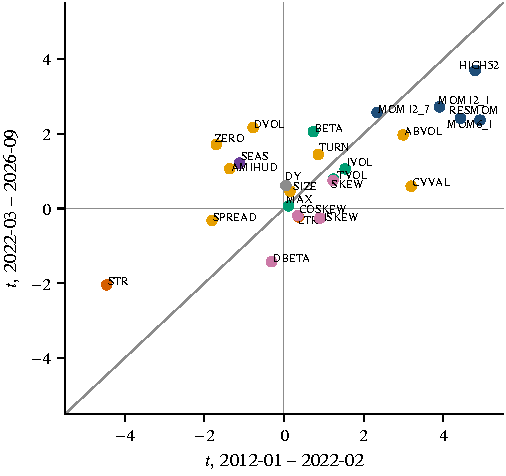
\includegraphics[width=0.55\linewidth]{figures/fig_regimes.pdf}
\caption{$t$-statistics of the 25 oriented long--short portfolios before (2012:01--2022:02) and after (2022:03--2026:09)
the exclusion of foreign investors, coloured by cluster. The diagonal marks equal $t$-statistics.}\label{fig:regimes}
\end{figure}

\subsection{Trading costs and implementability}\label{sec:costs}

Table~\ref{tab:costs} charges each trade one half of the \citet{abdi2017simple} close--high--low spread estimate for the
formation month plus 5 basis points of fees, and computes turnover from drifted weights. The resulting one-way cost
averages 35 to 40 basis points; the estimate is crude, and it ignores price impact. Momentum portfolios turn over
about one to one and a half times their notional a month (summing both legs), so the cost drag is 0.4 to 0.6
percentage points a month. I treat H5 as supported when the net mean is significantly positive at the 5\% level. All four momentum
survivors remain significant net of costs, so H5 holds for them under this cost model: the
52-week high ($t=\val{NetTHIGH52}$), six-month momentum ($t=\val{NetTMOM61}$), twelve-month momentum
($t=\val{NetTMOM121}$) and residual momentum ($t=\val{NetTRESMOM}$). They also survive an exploratory \RW{} test on net
returns, and they remain significant at conventional levels when costs are doubled. Their break-even one-way costs are
\val{BEHIGH52}, \val{BEMOM61}, \val{BEMOM121} and \val{BERESMOM} basis points, respectively. Abnormal volume, which
turns over about twice its notional a month, does not survive costs: its net mean, \val{NetMeanABVOL}\% a month, is
positive but insignificant ($t=\val{NetTABVOL}$), so H5 is not supported for it.

\paragraph{Implementability (exploratory).} The cost model covers spreads and fees only. Table~\ref{tab:implement}
examines what it leaves out: the availability and cost of short positions, the 2022 short-sale ban and price impact;
margin requirements and the financing of net positions are not modelled.
Historical data on which shares could be borrowed and at what fee are not available, so the table relies on proxies and
break-even values. Between \val{ImpShareMin} and \val{ImpShareMax}\% of each momentum premium comes from the long leg
(panel A): measured against the equal-weighted return of all sorted shares, the long leg of the 52-week-high portfolio
earns \val{ImpLongHIGH}\% a month ($t=\val{ImpLongTHIGH}$) and its short leg \val{ImpShortHIGH}\%
($t=\val{ImpShortTHIGH}$), a split close to the one \citet{israel2013role} report for US momentum. Restricting the short
leg to the 50 most liquid shares, or, from January 2013, the first holding month with an index base in force, to
constituents of the MOEX Russia index---rough proxies for the lists of shares that brokers allow clients to sell short---keeps all four momentum premia
significant net of spread costs ($t$ between \val{UfiftyTmin} and \val{UfiftyTmax}, and between \val{IdxTmin} and
\val{IdxTmax}). Replacing the short legs by cash
in the four months whose short positions would have been opened while short sales were banned, from 24 February to
31 May 2022 \citep{cbr2022shortban}, changes little. A borrow fee on
the short leg would have to exceed \val{BEfeeMin}--\val{BEfeeMax}\% a year to eliminate the net momentum premia; at
10\% a year the 52-week high and twelve-month momentum remain significant, six-month momentum is borderline and residual
momentum is not. Abnormal volume and short-term continuation, whose net premia are small to begin with, do not
survive a borrow fee of 10\% a year.

Price impact is the binding constraint. Under the square-root rule of thumb, in which a trade of $Q$ roubles in a share
with daily trading value $V$ and daily volatility $\sigma$ costs about $Y\sigma\sqrt{Q/V}$ with $Y$ of order one
\citep{toth2011anomalous}, the net premia of the equal-weighted momentum portfolios vanish at between \val{CapFullMin}
and \val{CapFullMax} million roubles per leg over the full sample with $Y=1$, and at between \val{CapHalfMin} and
\val{CapHalfMax} million with $Y=0.5$ (panel B). Most of the constraint comes from the early years. In 2012--2015 the
median U100 share traded about \val{ADVearlyMin}--\val{ADVearlyMax} million roubles a day and in 2023--2026
\val{ADVlateMin}--\val{ADVlateMax} million; over 2022--2026 the break-even sizes rise to between \val{CapPostMin}
million and \val{CapPostMax} billion roubles per leg with $Y=1$. These calculations are illustrative---the impact
coefficient is not estimated for MOEX, and each trade is assumed to be executed within a day---but they show that the
gross premia of equal-weighted portfolios overstate what an investor of meaningful size could have earned.

\begin{table}[!htbp]
\centering\small
\caption{Implementability of the survivors (exploratory)}\label{tab:implement}
\resizebox{\linewidth}{!}{\begin{tabular}{l rrr r r r r rr}
\toprule
\multicolumn{10}{l}{\emph{Panel A. Legs and short selling}} \\
 & & \multicolumn{2}{c}{Leg vs.\ all sorted} & & Break-even & Net, & Net, & \multicolumn{2}{c}{Net, shorts only in} \\
\cmidrule(lr){3-4}\cmidrule(lr){9-10}
 & Gross & Long & Short & Net & fee (\% p.a.) & fee 10\% & 2022 ban & U50 & Index$^{\ddagger}$ \\
\midrule
HIGH52 & 3.08 & 1.53 & 1.55 & 2.63 & 31.6 & 1.80 & 2.60 & 2.34 & 2.89 \\
 & (6.07) & (6.65) & (4.67) & (5.15) &  & (3.52) & (4.90) & (3.87) & (4.32) \\[1pt]
MOM6\_1 & 2.19 & 0.81 & 1.37 & 1.63 & 19.6 & 0.80 & 1.62 & 1.39 & 1.29 \\
 & (5.33) & (3.60) & (5.64) & (4.00) &  & (1.96) & (3.78) & (2.81) & (2.46) \\[1pt]
RESMOM & 1.64 & 0.86 & 0.78 & 1.24 & 14.9 & 0.41 & 1.26 & 1.23 & 1.27 \\
 & (4.90) & (3.90) & (4.07) & (3.75) &  & (1.23) & (3.64) & (3.13) & (3.21) \\[1pt]
MOM12\_1 & 2.28 & 1.01 & 1.26 & 1.90 & 22.8 & 1.07 & 1.91 & 1.72 & 1.93 \\
 & (4.72) & (4.70) & (3.99) & (3.97) &  & (2.23) & (3.86) & (3.38) & (3.67) \\[1pt]
ABVOL & 1.40 & 0.53 & 0.86 & 0.56 & 6.7 & $-$0.27 & 0.61 & 1.17 & 0.08 \\
 & (3.52) & (2.40) & (4.14) & (1.40) &  & ($-$0.68) & (1.56) & (2.09) & (0.14) \\[1pt]
STR$^{\dagger}$ & 1.96 & 0.77 & 1.19 & 0.82 & 9.9 & $-$0.01 & 0.84 & 0.53 & 0.54 \\
 & (4.96) & (3.07) & (5.70) & (2.00) &  & ($-$0.02) & (2.00) & (1.19) & (1.09) \\[1pt]
\bottomrule
\end{tabular}}\par\medskip
\resizebox{\linewidth}{!}{\begin{tabular}{l rr rr cc cc}
\toprule
\multicolumn{9}{l}{\emph{Panel B. Price impact (illustrative)}} \\
 & \multicolumn{4}{c}{Net return} & \multicolumn{4}{c}{Break-even size (RUB m per leg)} \\
\cmidrule(lr){2-5}\cmidrule(lr){6-9}
 & \multicolumn{2}{c}{RUB 0.1bn per leg} & \multicolumn{2}{c}{RUB 1bn per leg} & \multicolumn{2}{c}{$Y=1$} & \multicolumn{2}{c}{$Y=0.5$} \\
\cmidrule(lr){2-3}\cmidrule(lr){4-5}\cmidrule(lr){6-7}\cmidrule(lr){8-9}
 & 2012--26 & 2022--26 & 2012--26 & 2022--26 & 2012--26 & 2022--26 & 2012--26 & 2022--26 \\
\midrule
HIGH52 & 0.59 & 1.88 & $-$3.82 & 0.51 & 167 & 1{,}581 & 667 & 6{,}323 \\
 & (0.93) & (2.18) & ($-$3.48) & (0.49) & & & & \\[1pt]
MOM6\_1 & $-$0.91 & 0.00 & $-$6.40 & $-$1.93 & 41 & 101 & 165 & 404 \\
 & ($-$1.74) & (0.01) & ($-$6.10) & ($-$2.33) & & & & \\[1pt]
RESMOM & $-$0.61 & 0.29 & $-$4.60 & $-$1.02 & 45 & 219 & 180 & 875 \\
 & ($-$1.53) & (0.55) & ($-$5.57) & ($-$1.60) & & & & \\[1pt]
MOM12\_1 & 0.16 & 1.08 & $-$3.62 & $-$0.11 & 119 & 876 & 475 & 3{,}503 \\
 & (0.28) & (1.46) & ($-$4.07) & ($-$0.14) & & & & \\[1pt]
ABVOL & $-$3.48 & $-$0.65 & $-$12.21 & $-$3.42 & 2 & 24 & 8 & 97 \\
 & ($-$6.12) & ($-$0.80) & ($-$8.27) & ($-$2.75) & & & & \\[1pt]
STR$^{\dagger}$ & $-$4.81 & $-$1.27 & $-$16.98 & $-$5.38 & 2 & 11 & 9 & 44 \\
 & ($-$5.37) & ($-$1.17) & ($-$7.24) & ($-$3.06) & & & & \\[1pt]
\bottomrule
\end{tabular}}
\tabnote{Monthly means in \% with Newey--West $t$-statistics in parentheses, 2012:01--2026:09 unless stated. Panel A:
long (short) leg: return of the long leg minus (of all sorted shares minus the short leg), gross of costs, against the
equal-weighted return of all shares in the sort. Net: after the spread-based cost model of Section~\ref{sec:costs}.
Break-even fee: annual borrow fee on the short leg that sets the mean net return to zero. 2022 ban: short legs replaced
by cash in the holding months March--June 2022, whose portfolios are formed at the closes of February to May. U50, Index: the short leg holds only those shares of the short quintile
that are among the 50 most liquid, or in the MOEX Russia index base in force at the formation date; if no share of the short quintile is
eligible, the short leg holds all eligible shares in the sort. $^{\ddagger}$Holding months 2013:01--2026:09: the first base takes
effect in December 2012 and none is backfilled; over the same months the unrestricted net returns of the four momentum
portfolios have $t$ between \val{IdxWinTmin} and \val{IdxWinTmax}. Panel B: net return after
spread costs and a square-root impact charge $Y\sigma_i\sqrt{Q_i/V_i}$ per unit traded, where $Q_i$ is the rouble
amount traded, $V_i$ the mean daily trading value and $\sigma_i$ the daily volatility of share $i$ in the formation
month, with $Y=1$ unless stated. When fewer than 15 daily returns are available (as in the formation month March 2022),
$\sigma_i$ is the s.d.\ of at least five daily returns of the month, or else the share's value for the previous month. Because the charge is proportional to $Y\sqrt{A}$ for a
position of $A$ roubles per leg, the break-even size is $A^\ast=(\bar n/\bar c)^2$, where $\bar n$ is the mean net return
before impact and $\bar c$ the mean impact charge per unit of $\sqrt{A}$. 2022--26: holding months 2022:03--2026:09. STR$^{\dagger}$: the short-term continuation strategy (winners minus
losers of month $t$).}
\end{table}

\begin{table}[!htbp]
\centering\small
\caption{Trading costs}\label{tab:costs}
\resizebox{\linewidth}{!}{\begin{tabular}{l rrr rr rr r c}
\toprule
 & \multicolumn{3}{c}{Gross} & \multicolumn{2}{c}{Net (1$\times$ cost)} & \multicolumn{2}{c}{Net (2$\times$ cost)} & Break-even & RW net \\
\cmidrule(lr){2-4}\cmidrule(lr){5-6}\cmidrule(lr){7-8}
Factor & Mean & Turnover & Cost & Mean & $t$ & Mean & $t$ & (bp, one-way) & \\
\midrule
MOM12\_1 & 2.28 & 0.99 & 0.37 & 1.90 & 3.97 & 1.53 & 3.20 & 231 & \checkmark \\
MOM6\_1 & 2.19 & 1.46 & 0.56 & 1.63 & 4.00 & 1.07 & 2.64 & 150 & \checkmark \\
MOM12\_7 & 1.54 & 1.35 & 0.51 & 1.02 & 2.15 & 0.51 & 1.07 & 114 &  \\
RESMOM & 1.64 & 1.11 & 0.40 & 1.24 & 3.75 & 0.84 & 2.56 & 148 & \checkmark \\
HIGH52 & 3.08 & 1.23 & 0.45 & 2.63 & 5.15 & 2.19 & 4.22 & 252 & \checkmark \\
\addlinespace[2pt]
STR & $-$1.96 & 3.10 & 1.14 & $-$3.10 & $-$7.91 & $-$4.24 & $-$10.55 & -- &  \\
LTR & 0.08 & 0.78 & 0.29 & $-$0.20 & $-$0.49 & $-$0.49 & $-$1.16 & 10 &  \\
\addlinespace[2pt]
SEAS & $-$0.12 & 3.07 & 1.14 & $-$1.26 & $-$4.16 & $-$2.40 & $-$7.29 & -- &  \\
\addlinespace[2pt]
BETA & 0.69 & 0.71 & 0.31 & 0.38 & 0.83 & 0.07 & 0.15 & 97 &  \\
IVOL & 0.85 & 2.32 & 0.87 & $-$0.02 & $-$0.04 & $-$0.89 & $-$1.85 & 37 &  \\
TVOL & 0.72 & 2.32 & 0.90 & $-$0.18 & $-$0.36 & $-$1.08 & $-$2.13 & 31 &  \\
MAX & 0.06 & 2.69 & 1.04 & $-$0.97 & $-$2.00 & $-$2.01 & $-$4.05 & 2 &  \\
\addlinespace[2pt]
DBETA & $-$0.35 & 0.86 & 0.37 & $-$0.72 & $-$1.81 & $-$1.09 & $-$2.69 & -- &  \\
SKEW & 0.56 & 0.86 & 0.36 & 0.20 & 0.51 & $-$0.16 & $-$0.41 & 65 &  \\
ISKEW & 0.24 & 0.85 & 0.36 & $-$0.12 & $-$0.30 & $-$0.48 & $-$1.14 & 28 &  \\
COSKEW & 0.06 & 0.98 & 0.39 & $-$0.33 & $-$1.01 & $-$0.73 & $-$2.03 & 7 &  \\
\addlinespace[2pt]
SIZE & 0.18 & 0.38 & 0.13 & 0.05 & 0.11 & $-$0.09 & $-$0.20 & 48 &  \\
AMIHUD & $-$0.16 & 0.45 & 0.19 & $-$0.35 & $-$0.86 & $-$0.54 & $-$1.33 & -- &  \\
DVOL & 0.24 & 0.46 & 0.19 & 0.05 & 0.16 & $-$0.13 & $-$0.38 & 51 &  \\
TURN & 0.62 & 0.40 & 0.14 & 0.48 & 1.17 & 0.34 & 0.83 & 155 &  \\
ZERO & $-$0.32 & 0.68 & 0.26 & $-$0.58 & $-$1.28 & $-$0.84 & $-$1.85 & -- &  \\
SPREAD & $-$0.83 & 2.25 & 0.84 & $-$1.67 & $-$3.50 & $-$2.51 & $-$5.18 & -- &  \\
CVVAL & 0.98 & 0.79 & 0.30 & 0.68 & 1.90 & 0.38 & 1.04 & 124 &  \\
ABVOL & 1.40 & 2.08 & 0.84 & 0.56 & 1.40 & $-$0.27 & $-$0.66 & 67 &  \\
\addlinespace[2pt]
DY & 0.16 & 0.80 & 0.26 & $-$0.10 & $-$0.24 & $-$0.36 & $-$0.85 & 20 &  \\
\bottomrule
\end{tabular}}
\tabnote{Gross mean, net means and costs in \% per month. Turnover: average monthly sum over both legs of
$|w_{\text{new}}-w_{\text{drifted}}|$. One-way cost per share-month: half of the \citet{abdi2017simple} spread estimate
for the formation month plus 5 bp (cross-sectional median if unavailable). Break-even: one-way cost in basis points that
sets the mean net return to zero; ``--'' for negative gross means. RW net: discovery under the \RW{} rung for net
returns (exploratory). Newey--West $t$-statistics.}
\end{table}

\subsection{Fama--MacBeth regressions}\label{sec:fm}

Table~\ref{tab:fm} reports monthly cross-sectional regressions of next-month returns on cross-sectional ranks scaled to
$[-0.5,0.5]$ and oriented, so that a slope is the return spread between the highest- and lowest-ranked share
\citep{fama1973risk}. Univariate slopes reproduce the portfolio sorts (the 52-week high has $t=\val{FMtHIGHuni}$). When
all 25 ranks enter jointly, as the plan prescribes, no slope is significant (the largest $|t|$ is \val{FMmaxTmulti}):
the five momentum signals are collinear and share their explanatory power. Two exploratory specifications illustrate
this. With one canonical characteristic per cluster, twelve-month momentum ($t=\val{FMtMOMA}$) and short-term
continuation ($t=\val{FMtSTRA}$) are the only significant predictors. With the \RW{} survivors and short-term
continuation together, twelve-month momentum keeps $t=\val{FMtMOMB}$, the 52-week high $t=\val{FMtHIGHB}$ and
continuation $t=\val{FMtSTRB}$, while abnormal volume falls to $t=\val{FMtABVOLB}$. The momentum survivors are therefore
best read as heavily overlapping measurements of trend; abnormal volume partly overlaps with short-term continuation.

The time series of the portfolio returns agree (exploratory). The four momentum survivors have pairwise correlations
between \val{SurvCorrMin} and \val{SurvCorrMax}, and the first principal component of their correlation matrix accounts
for \val{SurvEigShare}\% of the total. Regressed on the other three, six-month momentum ($t(\alpha)=\val{SpanTMOM61}$)
and twelve-month momentum ($t(\alpha)=\val{SpanTMOM121}$) are spanned, while the 52-week high
($t(\alpha)=\val{SpanTHIGH52}$) and residual momentum ($t(\alpha)=\val{SpanTRESMOM}$) keep alphas that are significant
only at the conventional level. An equal-weighted composite of the four earns \val{CompMean}\% a month
($t=\val{CompT}$). Regressed on the 52-week high and residual momentum alone, six- and
twelve-month momentum have $t(\alpha)=\val{SpanTwoTMOM61}$ and $\val{SpanTwoTMOM121}$. Abnormal volume is nearly
uncorrelated with the momentum survivors (correlations of \val{SurvCorrAbvolMax} or less), and its alpha against them
has $t=\val{SpanTABVOL}$. These tests do not establish the exact number of distinct
effects, since an insignificant incremental alpha is also what weak power would produce, but they show that the four
survivors are largely redundant: the robust evidence is one momentum family, plus a fragile high-volume premium.

\begin{table}[!htbp]
\centering\small
\caption{Fama--MacBeth regressions}\label{tab:fm}
\resizebox{\linewidth}{!}{\begin{tabular}{l rr rr rr rr}
\toprule
 & \multicolumn{2}{c}{Univariate} & \multicolumn{2}{c}{All 25 jointly} & \multicolumn{2}{c}{One per cluster$^\ast$} & \multicolumn{2}{c}{Survivors + STR$^\ast$} \\
\cmidrule(lr){2-3}\cmidrule(lr){4-5}\cmidrule(lr){6-7}\cmidrule(lr){8-9}
Characteristic & Slope & $t$ & Slope & $t$ & Slope & $t$ & Slope & $t$ \\
\midrule
MOM12\_1 & 2.63 & 4.68 & 1.75 & 0.98 & 2.63 & 5.22 & 1.67 & 2.09 \\
MOM6\_1 & 2.23 & 4.60 & 0.49 & 0.42 &  &  & 0.06 & 0.10 \\
MOM12\_7 & 1.89 & 3.68 & 0.09 & 0.06 &  &  &  &  \\
RESMOM & 1.96 & 4.66 & 0.29 & 0.28 &  &  & 0.30 & 0.52 \\
HIGH52 & 3.45 & 6.23 & 0.98 & 1.07 &  &  & 1.32 & 1.76 \\
\addlinespace[2pt]
STR & $-$2.31 & $-$4.75 & $-$0.87 & $-$1.54 & $-$1.85 & $-$3.46 & $-$1.21 & $-$2.37 \\
LTR & 0.05 & 0.10 & 0.63 & 0.80 &  &  &  &  \\
\addlinespace[2pt]
SEAS & 0.09 & 0.26 & $-$0.46 & $-$0.98 & $-$0.30 & $-$0.87 &  &  \\
\addlinespace[2pt]
BETA & 0.89 & 1.80 & 1.28 & 1.53 & 0.43 & 0.56 &  &  \\
IVOL & 0.86 & 1.58 & 1.72 & 1.57 &  &  &  &  \\
TVOL & 0.93 & 1.61 & $-$0.05 & $-$0.04 &  &  &  &  \\
MAX & 0.29 & 0.52 & $-$1.00 & $-$1.05 &  &  &  &  \\
\addlinespace[2pt]
DBETA & $-$0.37 & $-$0.82 & 0.47 & 0.61 & 0.21 & 0.34 &  &  \\
SKEW & 0.50 & 1.12 & 0.31 & 0.29 &  &  &  &  \\
ISKEW & 0.34 & 0.71 & 0.33 & 0.32 &  &  &  &  \\
COSKEW & 0.20 & 0.56 & 0.51 & 0.91 &  &  &  &  \\
\addlinespace[2pt]
SIZE & 0.05 & 0.09 & 1.51 & 1.40 & 0.54 & 1.14 &  &  \\
AMIHUD & $-$0.33 & $-$0.70 & $-$0.95 & $-$0.50 &  &  &  &  \\
DVOL & 0.10 & 0.24 & 0.10 & 0.06 &  &  &  &  \\
TURN & 0.72 & 1.55 & 1.26 & 1.83 &  &  &  &  \\
ZERO & $-$0.34 & $-$0.72 & 0.03 & 0.06 &  &  &  &  \\
SPREAD & $-$0.85 & $-$1.59 & $-$0.27 & $-$0.68 &  &  &  &  \\
CVVAL & 1.00 & 2.52 & 0.48 & 0.83 &  &  &  &  \\
ABVOL & 1.52 & 3.49 & 0.42 & 0.98 &  &  & 0.46 & 1.02 \\
\addlinespace[2pt]
DY & 0.20 & 0.42 & 0.61 & 1.39 & 0.04 & 0.09 &  &  \\
\bottomrule
\end{tabular}}
\tabnote{Monthly cross-sectional OLS regressions in U100 of the month-$t+1$ return on cross-sectional ranks of the
characteristics scaled to $[-0.5,0.5]$ and oriented by the predicted sign; missing ranks are set to zero in the
multivariate regressions. Time-series averages of the slopes in \% per month with Newey--West $t$-statistics ($L=4$).
Univariate and ``All 25 jointly'' are pre-specified; columns marked $^\ast$ are exploratory.}
\end{table}

\subsection{Statistical power}

How much could fifteen years of Russian data reveal? I simulate samples of 177 months by resampling the demeaned
25-factor return matrix with the stationary bootstrap, which preserves the dependence and the tails, and inject a true
premium into one factor at a time. Table~\ref{tab:power} and Figure~\ref{fig:power} report the probability that the
injected factor is discovered, averaged over the 25 factors. A factor with an annual Sharpe ratio of 0.5 clears
$t>1.96$ about half the time but survives \RW{} with probability of only \val{PowRWsr0p5}; at 0.75 the \RW{} power is
\val{PowRWsr0p75}; at 1.0, \val{PowRWsr1p0}; and only at 1.25 does it exceed 0.9. The survivors have Sharpe ratios of
\val{SRsurvMin} to \val{SRsurvMax}, within the detectable range, although abnormal volume lies near its lower edge.
Many anomalies documented in the United States have long--short Sharpe ratios well below one, and the non-surviving
low-risk, size, liquidity and skewness portfolios here have Sharpe ratios between roughly $-0.4$ and $0.6$. Even the
conventional test detects a premium with a Sharpe ratio of 0.75 with probability \val{PowTsr0p75}. Premia that large
are therefore unlikely for the factors whose estimated Sharpe ratios are near or below zero, but not for the low-risk,
skewness and turnover portfolios, whose $t$-statistics lie between 1.4 and 1.9; and premia with Sharpe ratios of 0.5 or
less cannot be ruled out for any non-replicated factor. Their failure to replicate on MOEX is weak evidence against their
existence.

\begin{table}[!htbp]
\centering\small
\caption{Power of the ladder}\label{tab:power}
\begin{tabular}{c cccccc}
\toprule
True annual SR & R1 $t{>}1.96$ & R2 $t{>}3$ & R3 Holm & R4 BH & R5 BY & R6 RW \\
\midrule
0.25 & 0.18 & 0.04 & 0.03 & 0.04 & 0.02 & 0.03 \\
0.50 & 0.50 & 0.18 & 0.16 & 0.17 & 0.10 & 0.13 \\
0.75 & 0.81 & 0.48 & 0.45 & 0.45 & 0.33 & 0.39 \\
1.00 & 0.96 & 0.79 & 0.76 & 0.77 & 0.65 & 0.72 \\
1.25 & 0.99 & 0.94 & 0.93 & 0.94 & 0.89 & 0.91 \\
1.50 & 1.00 & 0.99 & 0.99 & 0.99 & 0.97 & 0.98 \\
\bottomrule
\end{tabular}
\tabnote{Probability that a single factor with the given true annualised Sharpe ratio is discovered (correct sign) when the
other 24 factors have zero premia. Samples of 177 months are drawn with the stationary bootstrap (mean block 6) from the
demeaned baseline factor returns; 300 outer resamples, each with 499 inner resamples for \RW{}; averages over the 25
factors.}
\end{table}

\begin{figure}[!htbp]
\centering
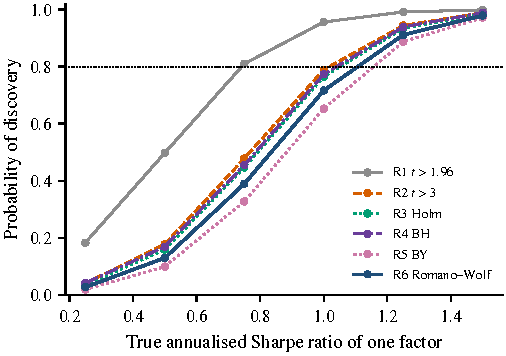
\includegraphics[width=0.6\linewidth]{figures/fig_power.pdf}
\caption{Probability of discovering one true factor as a function of its annualised Sharpe ratio, by rung.}\label{fig:power}
\end{figure}

% =====================================================================================
\section{Discussion}\label{sec:discussion}

\paragraph{What survives on MOEX.} The evidence supports one robust anomaly family: intermediate-horizon price momentum,
measured by past six- and twelve-month returns, residual returns or nearness to the 52-week high. These are largely
redundant measurements of one family, not four discoveries. The premia are large (Sharpe
ratios above one), survive the most demanding correction in nearly every full-sample variation of the protocol
(residual momentum in all of them), a size-calibrated version of that correction, bounds for unobserved delisting
losses, spread-based trading costs and restrictions of the short leg to liquid or index shares, and remain positive and
significant at conventional levels after 2022, although in the 55-month post-break sample no factor clears the \RW{}
bar. Their capacity in equal-weighted form is small, so the premia are better read as evidence about price formation
than as a measure of what a large investor could earn. Short-term continuation
among liquid shares is a second, less robust regularity: it passes the \RW{} test in eight of the eleven full-sample
specifications (not with value weights, in U50 or in UALL), and its net-of-cost return is borderline. Their cumulative returns (Figure~\ref{fig:cumret}) rise steadily except for a sharp momentum crash in February
2015, when the losers of the 2014 rouble crisis rebounded and twelve-month momentum lost \val{WorstAbsMOM121}\% in a month,
an episode of the kind described by \citet{daniel2016momentum}. The finding contrasts with the absence of momentum in
Eastern Europe over 1990--2011 reported by \citet{cakici2013size} and with the contrarian profits at longer horizons in
\citet{teplova2014momentum}, and it agrees with the significant momentum premium of \citet{ovechkin2022econometric} and
the after-cost momentum profits of \citet{nazarova2023momentum}. A market dominated by individual investors, with
short sales restricted at times of stress and episodic sanctions shocks, is a natural place for slow information
diffusion and under-reaction to persist.

\paragraph{What does not survive.} The implemented low-risk, size, liquidity, skewness, seasonality, long-term reversal
and dividend-yield signals do not survive in the liquid universe. For liquidity this matches \citet{teplova2022implicit}
and \citet{gurov2023illiquidity}, who find little cross-sectional evidence of an illiquidity premium on MOEX; for size it
matches \citet{ovechkin2022econometric}. Three qualifications limit what this means. The conclusion concerns these
implementations, which differ from several source definitions (Appendix Table~\ref{tab:adapt}); it concerns the 100 most
liquid shares, and the classic size and illiquidity premia do appear at the conventional level once the least liquid
shares are included (UALL); and it concerns a fifteen-year sample in which premia with Sharpe ratios of 0.5 or less would
be detected at most about half the time by the conventional test and rarely by the robust one. A failure to survive is
therefore weak evidence that an anomaly is absent from the Russian market.

\paragraph{Implications for empirical work on Russia and other emerging markets.} First, in samples of fifteen years
or less the familiar $t>3$ hurdle is not conservative enough: autocorrelation-robust $t$-statistics are more dispersed
than the normal distribution, and the bootstrap \RW{} critical value ranges from 3.3 to 3.6 across specifications and
approaches 4 in a 55-month subsample. Researchers working with short emerging-market histories should use bootstrap
critical values for the studentised statistics rather than normal $p$-values, and should check the size of the
bootstrap test by simulation, because even it is somewhat liberal at these sample lengths. Second, the closed-form Deflated Sharpe
Ratio should not be applied to a zoo of heterogeneous factors with the cross-factor variance of Sharpe ratios as its
benchmark; a bootstrap null benchmark gives sensible answers. Third, survivorship matters: about a third of the
shares that were ever among the 100 most liquid are no longer listed, and even a source that includes delisted shares can miss
delisted instruments of another type, as the depositary receipts missing here show. Fourth, Bayesian and frequentist replication
rates answer different questions; reporting both, as here, makes the difference explicit.

\begin{figure}[!htbp]
\centering
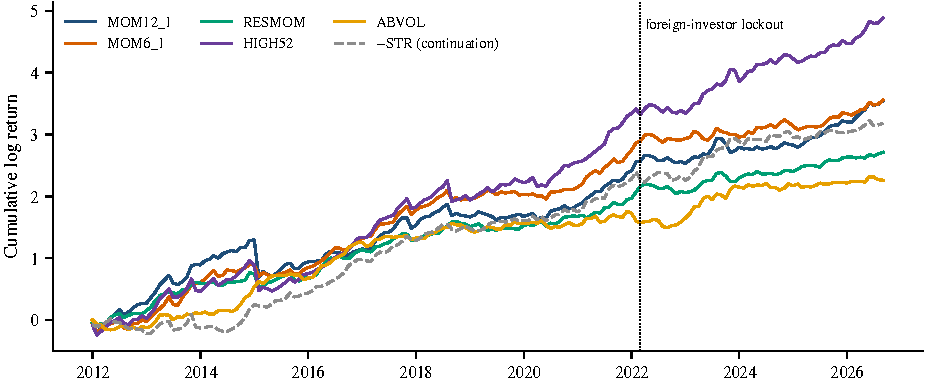
\includegraphics[width=\linewidth]{figures/fig_cumret.pdf}
\caption{Cumulative log returns of the five \RW{} survivors and of short-term continuation (the negative of the
reversal portfolio), baseline specification, 2012:01--2026:09. The dotted line marks the February 2022
suspension.}\label{fig:cumret}
\end{figure}

\paragraph{Limitations.} The study covers only characteristics that can be built from market data and dividends; the
value, profitability, investment and accrual families, which carry much of the US evidence, require accounting data
that are not available in open sources for the full cross-section including delisted firms. Market capitalisation is
point-in-time only for index constituents. Dividend coverage is thinner in the early years---the number of
dividend-paying securities recorded rises from 76 in 2010 to at least 100 in every year from 2011---which affects
only the formation windows of the longest-horizon characteristics in the first months; the momentum core survives
with price-only returns, so it does not hinge on dividends. Depositary receipts are covered only in part
(Section~\ref{sec:sources}). The final payoffs of delisted shares are not observed and are bounded rather than measured.
Historical data on which shares could be sold short and at what fee are not available, so the implementability
analysis relies on proxies; it does not model margin requirements or the financing of net positions, and its
price-impact calculation uses a rule of thumb rather than estimates for MOEX. And
the post-2022 sample is short.

% =====================================================================================
\section{Conclusion}\label{sec:conclusion}

A pre-specified test of 25 anomalies on fifteen years of Moscow Exchange share data free of survivorship bias finds
that
intermediate-horizon price momentum is the only anomaly family that survives a dependence-robust bootstrap correction
for multiple testing, nearly every variation of the protocol, bounds for unobserved delisting losses and spread-based
trading costs; its four surviving measures are largely redundant, and it remains significant at
conventional levels after the 2022 exclusion of foreign investors. Liquid Russian shares also exhibit short-term
continuation rather than reversal. The implemented low-risk, size, liquidity, skewness, seasonality and payout signals
do not survive, but the sample cannot reliably detect premia with Sharpe ratios much below one, so this is weak
evidence that those anomalies are absent. Methodologically, the Russian evidence shows that with fifteen years of
monthly data the bootstrap stepdown bar is higher than the familiar $t>3$ rule, because autocorrelation-robust
$t$-statistics are more dispersed than the normal distribution; corrections based on normal $p$-values therefore
overstate significance in samples of this length, and even the bootstrap test is somewhat liberal. Extending the zoo
to accounting-based characteristics, measuring short-sale costs and price impact on MOEX directly, and revisiting the
post-2022 regime as its sample lengthens are natural next steps.

\section*{Data availability}
All data are public. The replication package is available at \url{https://github.com/Sergpreneur/moex-factor-zoo}
(release v1.0). It contains the pre-analysis plan with its hash, timestamp and version history, the list of
deviations, the code that rebuilds every number, table and figure from the raw data, the monthly factor return series
(also as CSV files), the tests, and a provenance record of the data sources with their commit hashes; the raw data are
downloaded from their public sources by a script.

\section*{Declaration of generative AI and AI-assisted technologies in the writing process}
During the preparation of this work the author used Claude (Anthropic) to assist with code development, data processing
and drafting of the manuscript. The author reviewed and edited the content as needed and takes full responsibility for
the content of the publication.

\section*{Acknowledgements}
I thank the maintainers of the public MOEX data mirrors used in this study, in particular S.~Andreev for the
\texttt{moex-momentum} collection released under the MIT licence.

\FloatBarrier
\clearpage
\bibliographystyle{apalike}
\setstretch{1.0}
{\sloppy
\bibliography{references}}

\setstretch{1.25}
\appendix
\clearpage
\section{Deviations from the pre-analysis plan}\label{app:deviations}

\textbf{Implementation details not spelled out in the plan (decided before the factor results were seen).}
(i) When the Abdi--Ranaldo spread cannot be estimated for a share-month, its cost is set to the month's
cross-sectional median cost (50 basis points if no estimate exists). (ii) Abnormal volume requires at least six listed
months in the comparison window; all universes already require twelve months of trading, so the condition never binds.
(iii) The CAPM-alpha variant runs the ladder on market-hedged returns $r_{k,t}-\hat\beta_k(r_{m,t}-r_{f,t})$ with
$\hat\beta_k$ estimated once on the full sample; the bootstrap therefore ignores sampling error in $\hat\beta_k$.
(iv) Daily returns across gaps of more than 14 calendar days (the 2022 suspension) are excluded from daily statistics
for the market index as well as for shares. (v) The plan's characteristic table labels nine clusters, splitting downside
risk from skewness and size from liquidity, while its description of the empirical-Bayes model specifies seven; the
model uses seven, and the nine-label version gives the same replicated set (Section~\ref{sec:eb}).

\textbf{Changes made after the results were seen.} (vi) Bug fix: the MCFTRR series used here has no
print on 24 March 2022, so the daily market return on 25 March 2022 was first computed against the last pre-suspension
print, contrary to the 14-day rule.
It is now computed against the previous actual print and set to missing when the gap exceeds 14 days. The fix changes
the characteristics that use daily market returns (mainly beta, idiosyncratic skewness and co-skewness) in a few months;
it moves their baseline $t$-statistics by less than 0.05, and by at most 0.06 in any variant, and changes no discovery
count in any specification. (vii) The power study uses 300 common outer
resamples shared across the 25 factors and six Sharpe-ratio levels, with the inner \RW{} bootstrap computed once per
outer resample, instead of 100 independent outer replications per factor and level. Because the centred bootstrap
statistics are invariant to the injected drift, this changes the precision of the simulation, not its estimand.

\textbf{Exploratory analyses added after the results were seen.} (viii) The Deflated Sharpe Ratio with a bootstrap
null benchmark. (ix) Short-term returns within turnover terciles of UALL and turnover halves of U100
(Table~\ref{tab:str}). (x) The empirical-Bayes model without clusters and with nine clusters. (xi) Full ladders within
each regime. (xii) Two parsimonious Fama--MacBeth specifications (Table~\ref{tab:fm}). (xiii) The net-of-cost return of a
short-term continuation strategy and the \RW{} ladder on net returns. (xiv) The decomposition of the \RW{} critical
value in Section~\ref{sec:multiplicity} (Gaussian and i.i.d.\ Newey--West benchmarks with and without the factors'
correlation matrix, longer HAC lags, normal scores, rescaled bootstrap statistics, other seeds)
and the simulation of family-wise error control in Appendix~\ref{app:data}. (xv) Details of the PBO splits.

\textbf{Exploratory analyses added in the revision, after comments on the first version.} (xvi) Bounds for unobserved
delisting returns and a hold-to-resumption treatment of suspended shares (Section~\ref{sec:robust}). (xvii) U100 rebuilt
without the six depositary-receipt histories. (xviii) Residual momentum and idiosyncratic volatility with a
market-plus-SMB model. (xix) Long- and short-leg returns, break-even borrow fees, the 2022 short-sale ban, short legs
restricted to U50 or to index constituents, and an illustrative square-root price-impact charge
(Section~\ref{sec:costs}). (xx) Confidence intervals and minimum detectable changes for the regime differences, and the
regime comparison for the average of the momentum survivors. (xxi) Correlations and spanning regressions among the
survivors (Section~\ref{sec:fm}). (xxii) The simulation of family-wise error rates was enlarged from 1{,}000 to
\val{FWreps} replications per design and extended to Holm and the $t>3$ rule (the first version reported 6.2\% and
6.5\% for the \RW{} rung), and a size-calibrated \RW{} level was added (Section~\ref{sec:multiplicity}). (xxiii) A discrepancy with the plan, found in the revision: the plan states that depositary receipts are not in the
source and are therefore excluded, but six receipt histories are in the data and in the baseline universe
(\val{DRstockMonths} U100 stock-months from 2020). The baseline is kept as estimated; the universe that conforms to the
plan, without these six issuers, gives the same five survivors (Table~\ref{tab:revchecks}). The first version repeated
the plan's statement and described each characteristic as defined as in its source; Section~\ref{sec:sources} and
Table~\ref{tab:adapt} correct both. (xxiv) Added in a second revision: four data-construction sensitivities that
rebuild the panels from the raw data (a corrected dividend calendar; same-date payments treated as possible
duplicates; the dates of the Yahoo-derived dividend source moved two sessions earlier or later; Appendix~\ref{app:data}),
and a check of the volume-based characteristics for the shares that the price source takes from the T+2 board in 2013,
implemented in a separate module, so that the configuration and data-construction modules hashed at the freeze are
unchanged; look-ahead tests for universe membership and cost estimates and a continuity test of share counts through
splits; and the index-restricted short leg of Section~\ref{sec:costs} is now evaluated only from January 2013, the
first holding month with an index base in force (the first revision used the December 2012 base for earlier months).
None of these changes alters a pre-specified result.

Apart from item (xxiii), no characteristic, sign, window, universe, breakpoint, weighting scheme or sample period
differs from the plan.

\section{Data construction}\label{app:data}

\textbf{Sources and provenance.} Raw daily ISS share prices, the ticker dictionary including delisted securities,
dividends, splits
and MCFTRR are taken from the \texttt{moex-momentum} repository \citep{andreev2026moexmomentum} at commit
\texttt{240a69d}; MOEX index calculation bases and the key-rate history from the \texttt{moexutils} repository
\citep{moexutils} at commit \texttt{9742060}; the current MOEX list of securities from the \texttt{moex-dataset}
repository at commit \texttt{3320b44}. Prices in the first source are collected from every board on which a security
traded, with the main post-2013 board (TQBR) taking precedence over the legacy boards, which take precedence over the
odd-lot board. Dividends are collected from MOEX ISS and several secondary sources, reconciled, and checked for
completeness against MOEX's export of register-closing dates.

\textbf{Sessions.} The session calendar is the union of the dates on which MCFTRR is published and the dates on which at
least 20 shares traded (which adds official working Saturdays). Rows with non-positive closes or zero volume are
treated as days without trades.

\textbf{Dividends.} A share's payments with the same record date are summed. The data contain \val{DivGroupsAll}
such groups (\val{DivGroupsPairsAll} pairs and \val{DivGroupsTriples} triples); \val{DivPairs} of them, all pairs,
belong to shares that were ever in U100. Many are a final and an interim dividend declared together, as NLMK and
Severstal regularly do. I checked eight of the U100 pairs against issuer disclosures or press reports (NLMK
2015--2018, Severstal 2020, PIK and Inarctica 2021, Henderson 2024); all are distinct payments for different periods.
Treating every group as a possible duplicate and keeping only its largest payment (an exploratory sensitivity, built on
the corrected ex-date rule described below) drops \val{DedupDropped} payments, \val{DedupDroppedU} of them for shares
that were ever in U100. Relative to the corrected rule alone it changes \val{DedupOnlyChanged} U100 holding-month
returns and no $t$-statistic by more than \val{DedupOnlyMaxDt}; relative to the baseline, \val{DedupChanged} returns
change, no $t$-statistic moves by more than \val{DedupMaxDt}, and the \RW{} survivors are unchanged.

The plan's ex-date rule has two approximations. It locates the ex-date on the share's own trading days, so when a share
does not trade around the record date the payout can be credited a few sessions early, in three U100 cases in the
previous month. And it applies T0 settlement until September 2013, although from 25 March 2013 the source takes the prices of
some of the largest shares, such as Sberbank and LUKOIL, from the T+2 board (TQBR); four U100 payouts are therefore
placed two sessions late, within the same month. A corrected rule (exploratory) locates the ex-date on the exchange
calendar, reads the settlement regime from the board on which the share traded, and credits the payout on the first own
trading day on or after the ex-date. It changes \val{DivcalChanged} U100 holding-month returns, leaves the survivors
unchanged and moves no baseline $t$-statistic by more than \val{DivcalMaxDt}.

The Yahoo-derived source stores ex-dates whose convention is not uniform before September 2013. For Sberbank it gives
11 April 2012, the session before the record date of 12 April, and 12 April 2013, the session after the record date
of 11 April; under the settlement regimes of the boards that supply the prices, the ex-dates were 13 April 2012 (T0)
and 10 April 2013 (T+2). Both rules take the stored date as the ex-date. Moving every date of this source two sessions
earlier (an exploratory sensitivity) changes \val{YahooEarlyChanged} U100 holding-month returns, and moving every date
two sessions later changes \val{YahooLateChanged}: most only slightly, through the price at which the payout is
reinvested, and a few by moving a large payout into the adjacent month. In both cases the number of discoveries at every
rung of the ladder and the survivors are unchanged, and the survivors' $t$-statistics move by at most
\val{YahooMaxDtSurv}; the largest change, \val{YahooMaxDt}, is for \val{YahooMaxDtId}, whose baseline $t$-statistic is
$\val{YahooMaxDtBaseT}$. Each of the four data sensitivities rebuilds the panels, characteristics and baseline
portfolios from the raw data in separate folders and reruns the ladder (\texttt{scripts/09\_run\_data\_sensitivities.sh};
definitions in \texttt{moexzoo/variants.py}).

\textbf{Trading volume in 2013.} The board switch noted above also affects volumes: from 25 March 2013 the source takes
the daily rows of some large shares, volumes included, from the T+2 board, which carried a small part of their trading
until the main board moved to T+2 on 2 September 2013. The recorded trading value of Sberbank, LUKOIL and VTB in
April--August 2013 is \val{BoardValLo} to \val{BoardValHi}\% of its level in the first quarter, against
\val{BoardCtlLo} to \val{BoardCtlHi}\% for Gazprom and Norilsk Nickel, which remain on the legacy board.
In all, \val{BoardN} shares have rows from a T+ board in that window. Their volume-based characteristics are understated in 2013, and abnormal volume, which compares a month
with the preceding twelve, is distorted until August 2014. Setting the seven volume- and trading-based characteristics
(abnormal volume, turnover, trading value, Amihud illiquidity, the variability of trading value, the zero-return
proportion and the spread) of these shares to missing for formation months 2013:03--2014:08 (\val{BoardStockMonths}
U100 stock-months; an exploratory sensitivity, \texttt{scripts/05h\_board\_volume.py}) lowers the $t$-statistic of
abnormal volume from \val{TABVOL} to \val{BoardTABVOL} and raises its \RW{} adjusted $p$-value from \val{PrwABVOL} to
\val{BoardPrwABVOL}; the number of discoveries at every rung and the survivors are unchanged, and no $t$-statistic
moves by more than \val{BoardMaxDt}. Universe membership uses the median trading value over twelve months, which damps
the effect: Sberbank, LUKOIL, VTB and RusHydro stay in U100 throughout.

\textbf{Ticker changes.} ISS records ticker changes (for example, TCSG to T); the predecessor's history is stitched into
the successor's file, so the universe keeps only one of the two in any month. Redomiciliations create new securities
with separate histories (for example, YNDX to YDEX). Where the predecessor was a depositary receipt with a different
ticker (for example, FIVE to X5 or HHRU to HEAD), only the successor is in the data (Section~\ref{sec:sources}).

\textbf{Integrity tests.} The replication package contains tests that (i) perturb prices, dividends, trading data and
market returns after a formation month at four dates and verify that no characteristic changes; (ii) verify the continuity of adjusted prices around the 1:100
split of Norilsk Nickel (2024), the 5000:1 reverse split of VTB (2024) and the 1:100 split of Transneft preferred shares
(2024); (iii) verify the placement and amount of a Sberbank dividend on its ex-date; (iv) verify the alignment of
holding-period returns; (v) compare the Newey--West estimator and the Holm, Benjamini--Hochberg and Benjamini--Yekutieli
procedures with \texttt{statsmodels}; (vi) check the \RW{} implementation under a global null; (vii) perturb the trading
data after a formation month (monthly trading value, trading days and last-trade dates; daily prices) and verify that
universe membership and trading-cost estimates do not change; (viii) verify that adjusted share counts, and hence
capitalisations, are continuous through all \val{NsplitEvents} splits that fall in the monthly panel, and that no
adjusted share count changes by more than a factor of three from one month to the next (the continuity check is
informative for the \val{NsplitPit} splits with point-in-time index-base share counts on both sides; for the others the
fallback count does not change across the split); and (ix) verify that the module of data-construction sensitivities
reproduces the frozen adjustment exactly when given the plan's dividend rule. Tests (vii)--(ix) were added in the
second revision. A separate
simulation (\val{FWreps} replications in each of two designs, $B=499$ inner resamples; exploratory) estimates the
family-wise error rates of the \RW{} rung, Holm and the $t>3$ rule under the global null. For a multivariate-$t$
process with five degrees of freedom, AR(1) coefficient 0.1 and the empirical correlation matrix of the factors they are
\val{FWrwPar}\%, \val{FWholmPar}\% and \val{FWtthreePar}\%; for a stationary bootstrap of the demeaned factor returns,
\val{FWrwBoot}\%, \val{FWholmBoot}\% and \val{FWtthreeBoot}\%, against a nominal 5\% (Wilson 95\% intervals in
Section~\ref{sec:multiplicity}). The bootstrap test is mildly liberal at this sample length and the normal-theory
procedures more so. Under the global null a family-wise error occurs exactly when the first-step bootstrap $p$-value
of the largest $|t|$ is at or below the nominal level, so the simulated rate can be computed for any level. The
calibrated level is the largest attainable level at which the simulated rate does not exceed 5\%:
\val{FWalphaPar} in the parametric design and \val{FWalphaBoot} in the bootstrap design; the smaller is used.

\section{Additional results}\label{app:additional}

\begin{table}[H]
\centering\footnotesize
\setstretch{1.0}
\caption{Implementation relative to the source definitions}\label{tab:adapt}
\begin{tabularx}{\linewidth}{@{}l>{\raggedright\arraybackslash}p{2.7cm}>{\raggedright\arraybackslash}X>{\raggedright\arraybackslash}X@{}}
\toprule
ID & Source & Source definition & Implementation here \\
\midrule
MOM12\_1 & \citet{jegadeesh1993returns} & Past 3--12-month returns; overlapping holding periods of 3--12 months & Months $t-11$ to $t-1$ (month $t$ skipped) \\
MOM6\_1 & \citet{jegadeesh1993returns} & As above, six-month formation & Months $t-5$ to $t-1$ \\
MOM12\_7 & \citet{novymarx2012momentum} & Returns 12 to 7 months before the holding month & As in the source \\
RESMOM & \citet{blitz2011residual} & Fama--French three-factor residuals, 36-month estimation; residuals over months $-12$ to $-2$ summed and scaled by their volatility & CAPM residuals, 35-month estimation (no book equity, hence no value factor); market-plus-SMB version in Table~\ref{tab:revchecks} \\
HIGH52 & \citet{george2004week} & Price relative to the 52-week high; overlapping multi-month holding periods & As in the source, one-month holding \\
STR & \citet{jegadeesh1990evidence} & Prior-month return & As in the source \\
LTR & \citet{debondt1985overreact} & 36-month formation and holding periods & Months $t-35$ to $t-12$ \\
SEAS & \citet{heston2008seasonality} & Same-calendar-month returns at annual lags, effect lasting up to 20 years & Mean over annual lags 1--5 (at least two) \\
BETA & \citet{frazzini2014betting} & Betas from five-year correlations of three-day returns and one-year volatilities, shrunk towards one; beta-neutral, rank-weighted, leveraged portfolio & \citet{dimson1979risk} beta over 252 sessions; low-minus-high quintile spread, not beta-neutral (its CAPM alpha is the closer test) \\
IVOL & \citet{ang2006cross} & S.d.\ of daily Fama--French three-factor residuals, previous month & CAPM residuals; market-plus-SMB version in Table~\ref{tab:revchecks} \\
TVOL & \citet{ang2006cross} & S.d.\ of daily returns, previous month & As in the source \\
MAX & \citet{bali2011maxing} & Maximum daily return, previous month & As in the source \\
DBETA & \citet{ang2006downside} & Beta on days with below-mean market returns, one year of daily data; main evidence contemporaneous & Same estimator, used to predict next-month returns \\
SKEW & \citet{amaya2015realized} & Weekly realised skewness from five-minute returns & Skewness of daily returns over 252 sessions (no intraday data) \\
ISKEW & \citet{boyer2010expected} & Expected idiosyncratic skewness from a cross-sectional forecasting model & Historical skewness of daily CAPM residuals over 252 sessions \\
COSKEW & \citet{harvey2000conditional} & Standardised coskewness from 60 monthly returns & From 252 daily returns \\
SIZE & \citet{banz1981relationship} & Market value of equity & Log capitalisation; share counts partly not point-in-time (PIT variant) \\
AMIHUD & \citet{amihud2002illiquidity} & Mean daily $|r|$ per unit of dollar volume over a year & As in the source (rouble value, 252 sessions) \\
DVOL & \citet{brennan1998alternative} & Dollar trading volume & Log mean daily rouble value, 252 sessions \\
TURN & \citet{datar1998liquidity} & Share turnover over recent months & Rouble value over mean capitalisation, 12 months \\
ZERO & \citet{lesmond1999new}; \citet{bekaert2007liquidity} & Proportion of zero-return days, a transaction-cost measure; priced in emerging markets in the second source & Proportion of no-trade or zero-return sessions, 252 sessions \\
SPREAD & \citet{corwin2012simple}; \citet{amihud1986asset} & High--low spread estimator; spread premium in the second source & Estimator as in the first source, month $t$ \\
CVVAL & \citet{chordia2001trading} & Coefficient of variation of monthly dollar volume over 36 months & Over 12 months \\
ABVOL & \citet{gervais2001high} & Unusually high volume over a day or a week; returns over the following month & Mean daily value in month $t$ relative to months $t-12$ to $t-1$ \\
DY & \citet{litzenberger1979effect} & Dividend yield in cross-sectional CAPM regressions & Trailing 12-month gross dividends over price, payers only \\
\bottomrule
\end{tabularx}
\tabnote{Month $t$ is the formation month and $t+1$ the holding month. Whatever the holding rule of the source, every
portfolio here is an equal-weighted quintile spread in U100 held for one month (Section~\ref{sec:design}); ``as in the
source'' refers to the measure, not to the portfolio rule.}
\end{table}

\begin{table}[H]
\centering\small
\caption{$t$-statistics across specifications}\label{tab:robust_t}
\resizebox{\linewidth}{!}{\begin{tabular}{lrrrrrrrrrrr}
\toprule
Factor & Base & VW & U50 & UALL & Terc. & Lag & Ord. & Price & Ex-22 & PIT & Hedged \\
\midrule
MOM12\_1 & \textbf{4.72} & \textbf{3.77} & \textbf{3.60} & 3.58 & \textbf{4.55} & \textbf{4.51} & \textbf{4.86} & \textbf{4.06} & \textbf{4.64} & \textbf{4.72} & \textbf{4.95} \\
MOM6\_1 & \textbf{5.33} & 2.61 & 2.46 & 3.16 & \textbf{4.32} & \textbf{5.32} & \textbf{5.31} & \textbf{4.47} & \textbf{5.32} & \textbf{5.33} & \textbf{5.59} \\
MOM12\_7 & 3.24 & 2.88 & 2.78 & 2.47 & \textbf{3.59} & 3.12 & \textbf{3.48} & 2.82 & 3.14 & 3.24 & \textbf{3.44} \\
RESMOM & \textbf{4.90} & \textbf{4.04} & \textbf{3.85} & \textbf{3.85} & \textbf{4.41} & \textbf{4.92} & \textbf{5.06} & \textbf{4.70} & \textbf{4.78} & \textbf{4.90} & \textbf{4.99} \\
HIGH52 & \textbf{6.07} & \textbf{4.00} & \textbf{4.20} & 2.61 & \textbf{6.24} & \textbf{6.47} & \textbf{6.29} & \textbf{4.80} & \textbf{6.06} & \textbf{6.07} & \textbf{5.90} \\
\addlinespace[2pt]
STR & \textbf{$-$4.96} & $-$2.40 & $-$3.27 & 0.29 & \textbf{$-$4.32} & \textbf{$-$5.46} & \textbf{$-$4.95} & \textbf{$-$3.79} & \textbf{$-$4.97} & \textbf{$-$4.96} & \textbf{$-$4.73} \\
LTR & 0.19 & 0.81 & 0.67 & 0.89 & $-$0.10 & 0.52 & $-$0.21 & 0.89 & 0.34 & 0.19 & 0.16 \\
\addlinespace[2pt]
SEAS & $-$0.41 & $-$0.61 & $-$0.21 & 1.62 & 0.24 & $-$0.96 & $-$0.10 & $-$0.92 & $-$0.61 & $-$0.41 & $-$0.40 \\
\addlinespace[2pt]
BETA & 1.52 & 1.77 & 1.51 & 1.91 & 1.61 & 2.15 & 1.73 & 1.13 & 1.50 & 1.52 & 1.73 \\
IVOL & 1.85 & 0.47 & 1.13 & 0.25 & 1.77 & 1.93 & 1.93 & 1.53 & 1.87 & 1.85 & 2.16 \\
TVOL & 1.46 & 0.05 & 1.28 & 0.49 & 1.59 & 1.45 & 1.56 & 1.14 & 1.36 & 1.46 & 1.86 \\
MAX & 0.13 & $-$0.95 & 0.45 & 0.40 & 0.96 & $-$0.08 & 0.32 & 0.05 & 0.07 & 0.13 & 0.27 \\
\addlinespace[2pt]
DBETA & $-$0.89 & $-$1.65 & $-$1.37 & 0.23 & $-$0.61 & $-$0.93 & $-$1.29 & $-$0.78 & $-$0.77 & $-$0.89 & $-$1.04 \\
SKEW & 1.46 & $-$0.22 & 0.84 & $-$0.66 & 1.07 & 1.58 & 1.52 & 1.35 & 1.83 & 1.46 & 1.47 \\
ISKEW & 0.59 & 0.54 & 0.60 & $-$0.76 & 0.69 & 0.56 & 0.81 & 0.60 & 0.80 & 0.59 & 0.62 \\
COSKEW & 0.21 & $-$1.48 & $-$0.27 & 1.99 & 0.48 & 0.41 & $-$0.11 & 0.43 & 0.28 & 0.21 & 0.18 \\
\addlinespace[2pt]
SIZE & 0.41 & 0.77 & $-$1.24 & 2.45 & 0.24 & 0.56 & 0.22 & 0.85 & 0.37 & $-$0.25 & 0.40 \\
AMIHUD & $-$0.39 & 1.42 & $-$1.20 & 2.00 & $-$0.81 & $-$0.11 & $-$0.12 & 0.25 & $-$0.78 & $-$0.39 & $-$0.36 \\
DVOL & 0.70 & 1.58 & $-$0.36 & 3.11 & $-$0.10 & 1.22 & 0.85 & 1.36 & 0.37 & 0.70 & 0.81 \\
TURN & 1.52 & 1.25 & 0.94 & 1.12 & 1.74 & 1.82 & 1.61 & 1.46 & 1.29 & 0.35 & 1.93 \\
ZERO & $-$0.70 & $-$0.10 & $-$0.69 & 2.47 & $-$0.73 & $-$0.31 & $-$0.72 & $-$0.47 & $-$0.74 & $-$0.70 & $-$0.68 \\
SPREAD & $-$1.74 & 0.34 & $-$1.09 & $-$0.11 & $-$1.29 & $-$1.97 & $-$1.68 & $-$1.05 & $-$1.89 & $-$1.74 & $-$2.01 \\
CVVAL & 2.79 & 1.26 & 1.63 & $-$0.44 & 2.05 & 2.39 & 2.55 & 2.14 & \textbf{3.29} & 2.79 & 2.79 \\
ABVOL & \textbf{3.52} & \textbf{3.92} & 2.49 & 1.21 & \textbf{3.79} & 3.09 & \textbf{3.45} & 2.37 & \textbf{3.85} & \textbf{3.52} & \textbf{3.72} \\
\addlinespace[2pt]
DY & 0.37 & $-$0.61 & $-$0.25 & 1.24 & 0.32 & 0.15 & 0.96 & 0.05 & 0.26 & 0.37 & 0.43 \\
\bottomrule
\end{tabular}}
\tabnote{Newey--West $t$-statistics of the oriented long--short portfolios. Bold: rejection by the \RW{} rung of that
specification (either sign). Base: baseline; VW: capped value weights; U50, UALL: universes; Terc.: terciles; Lag:
one-session implementation lag; Ord.: preferred shares dropped when the ordinary share is in U100; Price: price-only
holding returns; Ex-22: excluding 2022:02 and 2022:03; PIT: point-in-time size and turnover; Hedged: market-hedged returns $r_{k,t}-\hat\beta_k(r_{m,t}-r_{f,t})$, whose
$t$-statistic differs slightly from the regression $t(\alpha)$ in Table~\ref{tab:baseline}.}
\end{table}

\begin{table}[H]
\centering\small
\caption{Empirical-Bayes posteriors}\label{tab:eb}
\resizebox{\linewidth}{!}{\begin{tabular}{ll r rrr r rr}
\toprule
 & & & \multicolumn{4}{c}{Clustered prior (pre-specified)} & \multicolumn{2}{c}{No clusters$^\ast$} \\
\cmidrule(lr){4-7}\cmidrule(lr){8-9}
Factor & Cluster & OLS mean & Post. mean & 2.5\% & 97.5\% & $P(\mu>0)$ & Post. mean & $P(\mu>0)$ \\
\midrule
MOM12\_1 & Momentum & 2.28 & 0.89 & 0.43 & 1.36 & 1.00 & 0.40 & 1.00 \\
MOM6\_1 & Momentum & 2.19 & 0.79 & 0.37 & 1.21 & 1.00 & 0.43 & 1.00 \\
MOM12\_7 & Momentum & 1.54 & 0.71 & 0.29 & 1.12 & 1.00 & 0.20 & 0.90 \\
RESMOM & Momentum & 1.64 & 0.82 & 0.41 & 1.23 & 1.00 & 0.47 & 1.00 \\
HIGH52 & Momentum & 3.08 & 0.83 & 0.41 & 1.25 & 1.00 & 0.46 & 1.00 \\
\addlinespace[2pt]
STR & Reversal & $-$1.96 & $-$0.20 & $-$0.57 & 0.17 & 0.15 & 0.04 & 0.60 \\
LTR & Reversal & 0.08 & $-$0.14 & $-$0.52 & 0.24 & 0.24 & 0.24 & 0.92 \\
\addlinespace[2pt]
SEAS & Seasonality & $-$0.12 & $-$0.00 & $-$0.40 & 0.39 & 0.49 & 0.10 & 0.74 \\
\addlinespace[2pt]
BETA & Low risk & 0.69 & $-$0.04 & $-$0.36 & 0.28 & 0.40 & 0.04 & 0.59 \\
IVOL & Low risk & 0.85 & 0.03 & $-$0.27 & 0.34 & 0.59 & 0.35 & 1.00 \\
TVOL & Low risk & 0.72 & $-$0.01 & $-$0.34 & 0.31 & 0.47 & 0.27 & 0.98 \\
MAX & Low risk & 0.06 & $-$0.10 & $-$0.43 & 0.22 & 0.26 & 0.08 & 0.72 \\
\addlinespace[2pt]
DBETA & Skewness/downside & $-$0.35 & 0.22 & $-$0.10 & 0.54 & 0.91 & 0.20 & 0.89 \\
SKEW & Skewness/downside & 0.56 & 0.30 & $-$0.05 & 0.64 & 0.95 & 0.49 & 1.00 \\
ISKEW & Skewness/downside & 0.24 & 0.17 & $-$0.13 & 0.48 & 0.87 & 0.24 & 0.96 \\
COSKEW & Skewness/downside & 0.06 & 0.21 & $-$0.13 & 0.54 & 0.89 & 0.22 & 0.91 \\
\addlinespace[2pt]
SIZE & Size/liquidity & 0.18 & 0.44 & 0.19 & 0.69 & 1.00 & 0.44 & 1.00 \\
AMIHUD & Size/liquidity & $-$0.16 & 0.40 & 0.14 & 0.65 & 1.00 & 0.28 & 0.97 \\
DVOL & Size/liquidity & 0.24 & 0.48 & 0.21 & 0.74 & 1.00 & 0.48 & 1.00 \\
TURN & Size/liquidity & 0.62 & 0.41 & 0.16 & 0.66 & 1.00 & 0.33 & 0.98 \\
ZERO & Size/liquidity & $-$0.32 & 0.39 & 0.14 & 0.65 & 1.00 & 0.31 & 0.97 \\
SPREAD & Size/liquidity & $-$0.83 & 0.36 & 0.11 & 0.62 & 1.00 & 0.15 & 0.83 \\
CVVAL & Size/liquidity & 0.98 & 0.39 & 0.16 & 0.63 & 1.00 & 0.40 & 0.99 \\
ABVOL & Size/liquidity & 1.40 & 0.46 & 0.20 & 0.71 & 1.00 & 0.38 & 0.99 \\
\addlinespace[2pt]
DY & Payout & 0.16 & 0.14 & $-$0.32 & 0.59 & 0.72 & 0.25 & 0.93 \\
\bottomrule
\end{tabular}}
\tabnote{OLS mean and posterior moments of the oriented monthly premium (\%). Clustered prior: $\mu_k=\mu_0+c_{j(k)}+w_k$
with the seven clusters of Table~\ref{tab:defs}; hyperparameters by maximum marginal likelihood. No clusters: a single
exchangeable prior (exploratory).}
\end{table}

\begin{figure}[H]
\centering
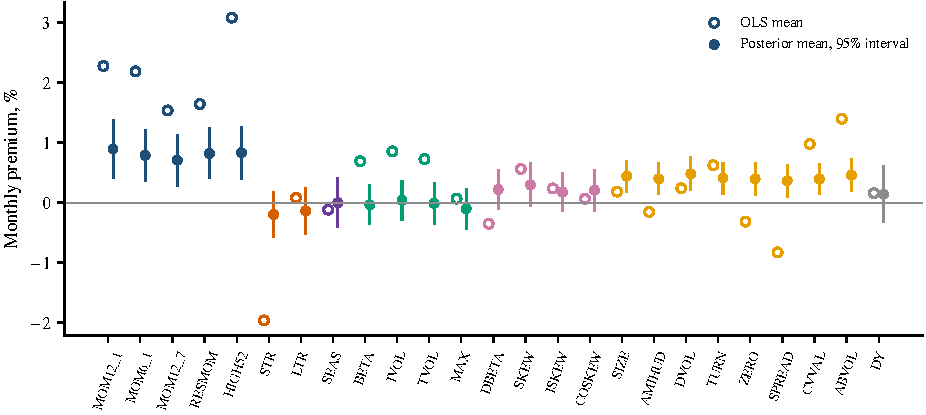
\includegraphics[width=\linewidth]{figures/fig_eb.pdf}
\caption{OLS means (open circles) and empirical-Bayes posterior means with 95\% intervals (filled), clustered prior.}\label{fig:eb}
\end{figure}

\begin{figure}[H]
\centering
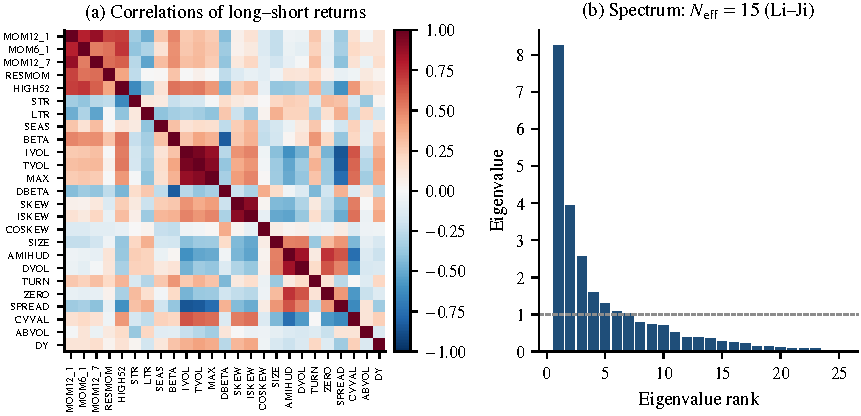
\includegraphics[width=\linewidth]{figures/fig_corr.pdf}
\caption{Correlations of the 25 oriented long--short returns (panel a) and the eigenvalues of their correlation matrix
(panel b).}\label{fig:corr}
\end{figure}

\end{document}
